\documentclass[12pt]{report}
\usepackage[utf8]{inputenc}
\usepackage[T1]{fontenc}
\usepackage[spanish,es-nodecimaldot,es-noshorthands]{babel}
\usepackage{setspace}
\usepackage{geometry}
\usepackage{hyperref}
\usepackage{amsmath}
\usepackage{amssymb}
\usepackage{graphicx}
\usepackage{csquotes}
\usepackage{float}

\geometry{letterpaper, margin=1in}

\title{Capítulos 1 y 2}
\author{José Manuel Martínez Durán}
\date{Junio 2026}

\begin{document}

% --- PÁGINA DE DERECHOS DE AUTOR ---
\newpage
\thispagestyle{empty}
\vspace*{\fill}
\begin{center}
\doublespacing
Derechos de autor \\
por \\
José Manuel Martínez Durán \\
2026
\end{center}
\vspace*{\fill}
\newpage

% --- PÁGINA EN BLANCO ---
\thispagestyle{empty}
\mbox{}
\newpage

% --- PÁGINA DE TÍTULO / DISERTACIÓN ---
\thispagestyle{empty}
\begin{center}
\doublespacing
\textbf{Inteligencia artificial generativa paramétrica aplicada a la \\ composición musical} \\
\vspace{1em}
por \\
\vspace{1em}
\textbf{José Manuel Martínez Durán, MVR} \\
\vspace{2em}
Disertación \\
Presentada a la División de Posgrado de \\
La Universidad Da Vinci \\
en cumplimiento parcial \\
de los requisitos \\
para la obtención del grado de \\
Doctorado en Ingeniería en Sistemas Computacionales \\
\vspace{2em}
Universidad Da Vinci \\
Febrero 2026
\end{center}
\vspace*{\fill}
\newpage

% --- PÁGINA DE APROBACIÓN ---
\thispagestyle{empty}
\begin{center}
\doublespacing
Inteligencia artificial generativa paramétrica aplicada a la \\ composición musical \\
\vspace{2em}
Aprobada por \\
Comité de Disertación: \\
\vspace{1em}
Dr. Agustin Santiago Alvarado, Supervisor \\
Dr. Pedro Damián Reyes \\
Dr. José Aníbal Arias Aguilar
\end{center}
\newpage

% --- PÁGINA EN BLANCO ---
\thispagestyle{empty}
\mbox{}
\newpage

% --- RESUMEN ---
\newpage
\begin{center}
\doublespacing
\textbf{Inteligencia artificial generativa paramétrica aplicada a la \\ composición musical} \\
\vspace{1em}
\textbf{José Manuel Martínez Durán, DSC} \\
Universidad Da Vinci, 2026 \\
Supervisor: Agustín Santiago Alvarado
\end{center}
\vspace{1em}
\begin{quote}
\doublespacing
Resumen: La presente investigación, aborda una problemática en el campo de la composición musical asistida por inteligencia artificial: la falta de control determinista y coherencia teórica en los modelos actuales. Los sistemas contemporáneos, basados mayoritariamente en el procesamiento de señales de audio o modelos de lenguaje secuenciales, operan como "cajas negras" que impiden la parametrización de variables estructurales esenciales como la tonalidad y el modo. Además, su salida en formato de audio dificulta la edición profesional, ignorando las reglas de la armonía funcional y el contrapunto inherentes al razonamiento humano.

El objetivo central es \textit{evaluar en qué medida una arquitectura híbrida de aprendizaje automático, sustentada en un sistema de representación matricial relativa, permite la generación de composiciones musicales simbólicas, paramétricas y estructuralmente coherentes}. La propuesta se fundamenta en tres pilares tecnológicos: Algoritmos Genéticos para la evolución de estilos basados en la preferencia del compositor; Árboles de Decisión que actúan como filtros deterministas para imponer restricciones técnicas "duras" (evitando errores como quintas paralelas o resoluciones incorrectas) ; y Redes Neuronales como generadores primarios de material melódico y armónico.
\end{quote}
\vspace*{\fill}
\newpage

% --- ÍNDICES ---
\tableofcontents \newpage
\listoftables \newpage
\listoffigures \newpage

% --- CUERPO DEL DOCUMENTO ---
\doublespacing

\chapter{Planteamiento del Problema}

\section{Definición del Problema}
En los últimos años, los Modelos de Lenguaje de Gran Escala (LLM, por sus siglas en inglés) han transformado radicalmente el panorama de la Inteligencia Artificial, democratizando la creación de contenido en diversos dominios \cite{sengar2025}. En el ámbito musical, esta tendencia ha dado lugar a plataformas que generan composiciones completas a partir de descripciones textuales, tales como Suno o Udio, e incluso modelos capaces de transformar tarareos informales en arreglos instrumentales complejos o sintetizar voces que interpretan letras específicas con un realismo sorprendente \cite{wei2024}. No obstante, a pesar de su impacto mediático y su utilidad en la industria publicitaria y de contenidos rápidos, la mayoría de estos sistemas se centran en la producción de audio final (forma de onda), omitiendo la generación de notación musical simbólica editable. Esta carencia limita su uso en la composición profesional, donde la precisión técnica y la posibilidad de refinamiento mediante partituras son fundamentales \cite{batlle2024}.

Los modelos actuales de Inteligencia Artificial Generativa Musical, predominantemente basados en el procesamiento de señales de audio o modelos de lenguaje secuenciales, presentan limitaciones significativas para su integración en flujos de trabajo de composición profesional. Estos sistemas operan frecuentemente como "cajas negras" que impiden la parametrización explícita de variables estructurales críticas, tales como tonalidad, métrica, modo y función armónica \cite{fernandez2023}.

Adicionalmente, la salida de estos modelos suele ser en formato de onda de audio, lo que obstaculiza su edición y requiere procesos complejos de transcripción para su uso instrumental. Desde la perspectiva del entrenamiento, las representaciones de datos utilizadas (formas de onda o secuencias planas de notas) no capturan la semántica profunda de la música, ignorando las reglas de la armonía funcional y el contrapunto inherentes al razonamiento de un compositor humano \cite{kaliakatsos20}.

\section{Preguntas de Investigación}

\subsection{Pregunta General}
¿En qué medida una arquitectura híbrida de aprendizaje automático, entrenada mediante un sistema de representación matricial relativa de armonía funcional, permite la generación de composiciones musicales paramétricas y estructuralmente coherentes?

\subsection{Preguntas Específicas}
\begin{itemize}
    \item ¿Cómo mejora la representación matricial relativa la capacidad del modelo para aprender y replicar funciones armónicas y contrapuntísticas en comparación con representaciones absolutas lineales?
    \item ¿De qué manera la integración de árboles de decisión y algoritmos genéticos permite controlar eficazmente los parámetros de composición (tonalidad, modo, métrica) sobre la salida generativa?
    \item ¿Cómo afecta la imposición de restricciones estrictas (reglas de armonía) mediante árboles de decisión a la creatividad o varianza de las melodías generadas por el algoritmo genético?
\end{itemize}

\section{Propósito y Objetivos del Estudio}
El propósito fundamental de esta investigación es cerrar la brecha entre la generación estocástica de audio y la composición técnica profesional. El objetivo general busca desarrollar y validar una arquitectura híbrida de inteligencia artificial que, mediante el uso de representaciones matriciales relativas, garantice la generación de música simbólica estructuralmente coherente y teóricamente correcta, enfocada en un usuario compositor musical.

Para alcanzar esto, los objetivos específicos se centran en tres etapas críticas: 
\begin{enumerate}
\item Formalizar matemáticamente el algoritmo de conversión matricial, asegurando que la jerarquía armónica sea capturada fielmente.

\item Implementar un sistema modular que integre redes neuronales para la creatividad melódica con árboles de decisión para el rigor técnico y algoritmos genéticos para la evolución estilística.

\item Realización de un análisis comparativo exhaustivo que contraste la salida del sistema propuesto frente a modelos tradicionales, evaluando la reducción de errores armónicos.
\end{enumerate}

\section{Justificación de la Investigación}
La relevancia de este estudio se sustenta en la transición necesaria de la inteligencia artificial como una herramienta de generación cerrada hacia un asistente creativo transparente y controlable. Actualmente, la industria musical demanda soluciones que no solo produzcan resultados estéticamente agradables, sino que respeten las leyes de la armonía funcional y el contrapunto, permitiendo a los compositores interactuar con el modelo en un nivel semántico profundo. Esta investigación aborda la problemática de la "caja negra" en los modelos generativos mediante una arquitectura híbrida que combina la potencia probabilística de las redes neuronales con la precisión lógica de los sistemas basados en reglas y la optimización de los algoritmos evolutivos.

Al introducir la representación matricial relativa, se proporciona un marco de datos que entiende la música como un sistema de sintaxis lógica y no solo como una sucesión estadística de notas. Esto no solo posee un valor científico al proponer nuevas estructuras de datos para el aprendizaje profundo en contextos artísticos, sino que también ofrece una utilidad práctica inmediata: la capacidad de generar archivos MIDI editables que cumplen con estándares académicos rigorosos. Esto facilita el flujo de trabajo en estudios de grabación, orquestación cinematográfica y desarrollo de videojuegos, donde la coherencia estructural es innegociable y la IA debe actuar como un colaborador competente y no como un generador aleatorio.

\section{Implicaciones y Delimitaciones}
\begin{itemize}
    \item \textbf{Diseño e Implementación de la Arquitectura Híbrida:} La investigación abarca el diseño, desarrollo y validación técnica de un sistema de software que integra algoritmos genéticos para la selección del estilo predilecto, árboles de decisión para la imposición de reglas estrictas de armonía y contrapunto, y redes neuronales para la generación de material melódico alternativo.
    \item \textbf{Validación de la Representación Matricial Relativa:} El estudio se centra en la propuesta de un nuevo algoritmo de representación basado en matrices relativas. Se evaluará su efectividad comparativa frente a representaciones lineales en términos de retención de contexto armónico.
    \item \textbf{Generación Simbólica y Parametrización:} El sistema se limita a la generación de salidas MIDI, permitiendo la manipulación de variables como tonalidad, modo y métrica.
    \item \textbf{Dominio de la Armonía:} La evaluación de coherencia se circunscribe a la armonía funcional occidental y el contrapunto estricto. Se evaluará la capacidad para evitar errores técnicos como quintas paralelas o resoluciones incorrectas de tritonos.
    \item \textbf{Exclusiones:} No se contemplan métricas estéticas subjetivas ni la generación automática de partituras visuales a partir del MIDI.
\end{itemize}

\chapter{Marco Teórico y Revisión de la Literatura}
\section{Fundamentos de la Música Simbólica y Teoría Musical}
\subsection{La música como sistema de eventos discretos}

La música puede entenderse como un sistema estructurado de eventos discretos organizados en el tiempo. A diferencia de fenómenos continuos como el ruido ambiental o ciertos procesos físicos naturales, la música en la tradición occidental se construye a partir de unidades diferenciables: notas con alturas específicas, duraciones definidas y relaciones jerárquicas dentro de escalas y acordes. Esta discretización permite representar, analizar y transmitir la música mediante sistemas simbólicos como la notación musical. En particular, la música diatónica constituye uno de los sistemas más influyentes en la historia de la teoría musical occidental, ya que establece un conjunto finito de relaciones entre alturas que pueden combinarse para formar melodías y armonías coherentes \cite{tymoczko2011}.

Desde una perspectiva histórica, el origen del pensamiento musical basado en relaciones discretas puede rastrearse hasta la antigua Grecia. Filósofos como Pitágoras observaron que ciertas proporciones numéricas simples entre longitudes de cuerdas producían intervalos que el oído percibía como consonantes. Por ejemplo, la relación 2:1 corresponde a la octava, mientras que 3:2 corresponde a la quinta justa \cite{baker2007}. Estas observaciones condujeron a la idea de que la música posee una estructura matemática subyacente basada en proporciones entre frecuencias. Este enfoque influyó profundamente en la teoría musical medieval y renacentista, donde la organización de los sonidos se interpretaba como un reflejo del orden matemático del universo \cite{christensen2002}. 

En términos físicos, el sonido es una onda mecánica que se propaga a través de un medio, usualmente el aire, como variaciones de presión. Una propiedad fundamental del sonido es su frecuencia, medida en Hertz (Hz), que representa el número de ciclos de vibración por segundo. La percepción humana del tono está estrechamente relacionada con la frecuencia de la onda sonora: frecuencias más altas se perciben como sonidos más agudos, mientras que frecuencias más bajas se perciben como sonidos más graves. En música, las alturas de los sonidos se organizan en un conjunto discreto de valores llamados notas\cite{zwicker2013}.

Las notas musicales constituyen representaciones simbólicas de alturas específicas. En el sistema musical occidental moderno, las notas se nombran utilizando las sílabas do, re, mi, fa, sol, la y si, que corresponden aproximadamente a las letras C, D, E, F, G, A y B en el sistema anglosajón. Estas notas no representan frecuencias únicas universales, sino posiciones relativas dentro de un sistema de afinación. Por ejemplo, en el sistema de afinación estándar contemporáneo, la nota La central (A4) se fija convencionalmente en 440 Hz , y las demás notas se calculan en relación con ella utilizando el sistema de temperamento igual \cite{iso16:1975}.

El temperamento igual divide la octava en doce intervalos iguales llamados semitonos. Matemáticamente, cada semitono corresponde a multiplicar la frecuencia anterior por el factor $2^{1/12}$ \cite{benson2006}. De esta forma, después de doce pasos se alcanza exactamente el doble de la frecuencia inicial, es decir, una octava. Este sistema permite modular entre tonalidades diferentes sin alterar significativamente las relaciones armónicas percibidas, lo cual fue fundamental para el desarrollo de la música tonal entre los siglos XVII y XIX \cite{isacoff2001temperament}.

En el contexto de este sistema, se distinguen dos tipos básicos de intervalos entre notas adyacentes: el tono y el semitono. Un semitono representa la distancia mínima entre dos notas dentro del sistema cromático de doce divisiones de la octava. Un tono equivale a dos semitonos. La escala diatónica se construye mediante una secuencia específica de tonos y semitonos que organiza siete notas dentro de la octava. La escala mayor, por ejemplo, sigue el patrón:
\begin{figure}[h]
\centering
\[
T - T - S - T - T - T - S
\]
\caption{Patrón de tonos (T) y semitonos (S) de la escala mayor diatónica}
\end{figure}
donde $T$ representa un tono y $S$ un semitono \cite{agmon1989diatonic}.

A partir de esta estructura surge la escala diatónica mayor, que constituye la base de gran parte de la música tonal occidental. Por ejemplo, la escala de Do mayor se compone de las notas:
\begin{figure}[h]
\centering
\[
C \; D \; E \; F \; G \; A \; B \; C
\]
\caption{Escala de Do mayor \cite{krumhansl1982spatiotemporal}}
\end{figure}


Esta escala es particularmente significativa porque puede representarse utilizando únicamente las teclas blancas del piano, lo que facilita su comprensión pedagógica. 

\begin{figure}[htbp]
    \centering
    \begin{center}
        \includegraphics[width=0.5\textwidth]{img/teclado.png} 
    \end{center}
    \caption{Teclado con escala de Do Mayor \cite{sudnow2001ways}}
    \label{fig:teclado_do_mayor} % Añadir una etiqueta para referencias cruzadas
\end{figure}


Las escalas no solo organizan alturas, sino que también establecen funciones tonales entre las notas. Dentro de la escala, cada grado tiene un papel específico en la percepción de estabilidad o tensión musical. Por ejemplo, el primer grado (tónica) actúa como centro tonal, mientras que el quinto grado (dominante) genera una sensación de tensión que tiende a resolverse hacia la tónica. Este sistema jerárquico constituye la base del lenguaje armónico de la música tonal \cite{riemann1893simplified}.

A partir de las escalas se construyen estructuras armónicas más complejas llamadas acordes. El tipo más fundamental de acorde es la tríada, que consiste en tres notas separadas por intervalos de tercera. Una tríada se forma tomando una nota de la escala (la fundamental), añadiendo la tercera y la quinta correspondientes dentro de la misma escala. Por ejemplo, la tríada construida sobre la nota Do en la escala de Do mayor está formada por \cite{piston1987harmony}:

\begin{figure}[h]
\centering
\[
C - E - G
\]
\caption{Triada de Do mayor}
\end{figure}

Esta combinación produce el acorde de Do mayor. Dependiendo de la relación entre los intervalos, las tríadas pueden clasificarse en diferentes tipos: mayor, menor, disminuida o aumentada. Una tríada mayor se caracteriza por contener una tercera mayor seguida de una tercera menor, mientras que una tríada menor contiene una tercera menor seguida de una tercera mayor.

\begin{figure}[htbp]
    \centering
    \begin{center}
        \includegraphics[width=0.5\textwidth]{img/triadas.png} 
    \end{center}
    \caption{Contruccion de la triada mayor y menor \cite{schoenberg1978}}
    \label{fig:teclado_do_mayor} % Añadir una etiqueta para referencias cruzadas
\end{figure}


Los acordes pueden ampliarse agregando notas adicionales como la séptima, la novena o la oncena, lo que da lugar a estructuras armónicas más complejas. Sin embargo, incluso en estos casos, la tríada continúa siendo el núcleo estructural del acorde. Esta organización jerárquica refleja nuevamente la naturaleza discreta de la música tonal: cada acorde pertenece a un conjunto finito de configuraciones posibles derivadas de la escala \cite{forte1982introduction} .

Desde un punto de vista analítico, el sistema diatónico puede entenderse como una red combinatoria de eventos discretos. Las notas constituyen los elementos básicos; los intervalos definen las relaciones entre ellos; las escalas organizan subconjuntos específicos de notas; y los acordes emergen como combinaciones estructuradas dentro de estas escalas. Esta perspectiva permite modelar la música utilizando herramientas matemáticas, teoría de conjuntos o grafos, enfoques que han sido explorados extensamente en la musicología computacional y la teoría musical contemporánea \cite{mazzola2012topos}.

\begin{figure}[htbp]
    \centering
    \begin{center}
        \includegraphics[width=0.5\textwidth]{img/quintas.png} 
    \end{center}
    \caption{Relaciones armónicas y círculo de quintas \cite{chew2014mathematical}}
    \label{fig:teclado_do_mayor} % Añadir una etiqueta para referencias cruzadas
\end{figure}

El círculo de quintas es otro concepto central que ilustra la organización discreta de las tonalidades. En este diagrama, cada tonalidad se conecta con otras mediante intervalos de quinta justa. Este arreglo revela patrones de proximidad tonal y facilita la comprensión de fenómenos como la modulación. Además, muestra cómo las doce notas del sistema cromático pueden organizarse en una estructura cíclica que refleja relaciones armónicas fundamentales \cite{krumhansl1990cognitive}.

Históricamente, el desarrollo del sistema diatónico estuvo ligado a la evolución de los sistemas de afinación. Durante la Edad Media y el Renacimiento se utilizaron diversos temperamentos basados en quintas puras o proporciones justas. Sin embargo, estos sistemas presentaban limitaciones al modular entre tonalidades distantes. El temperamento igual, adoptado progresivamente entre los siglos XVII y XVIII, resolvió estas limitaciones al distribuir uniformemente los intervalos dentro de la octava \cite{duffin2007how}.

En conclusión, la música diatónica puede describirse como un sistema estructurado de eventos discretos organizados jerárquicamente. Las frecuencias físicas del sonido se discretizan en notas; las notas se organizan en escalas mediante patrones específicos de intervalos; y las escalas generan acordes que constituyen la base de la armonía tonal. Este proceso de discretización no solo facilita la notación y transmisión de la música, sino que también permite su análisis mediante herramientas matemáticas y computacionales. La comprensión de estos elementos fundamentales es esencial para estudiar tanto la teoría musical tradicional como sus aplicaciones contemporáneas en campos como la musicología computacional, la inteligencia artificial musical y el análisis algorítmico de composiciones.


\subsection{Teoría de la Armonía Funcional, Contrapunto y Modos griegos}

La teoría musical occidental ha desarrollado múltiples marcos conceptuales para describir la organización de los sonidos en el tiempo. Entre los más influyentes se encuentran la armonía funcional, el contrapunto y el sistema modal heredado de la tradición griega y medieval. Estos enfoques describen diferentes dimensiones del lenguaje musical: la armonía funcional se ocupa de las relaciones jerárquicas entre acordes dentro de una tonalidad; el contrapunto estudia la interacción entre líneas melódicas independientes; y los modos proporcionan sistemas alternativos de organización de las alturas. En conjunto, estos conceptos constituyen una base teórica fundamental para comprender la estructura de la música tonal y modal \cite{delamotte1991harmony}.

\subsubsection{Armonía funcional}

La armonía funcional describe el papel que desempeñan los acordes dentro de una tonalidad. En este sistema, cada acorde derivado de una escala diatónica adquiere una función específica relacionada con la estabilidad o la tensión armónica. Las funciones principales son tres: tónica (T), dominante (D) y subdominante (S).

La tónica representa el centro tonal y el punto de reposo armónico. En la escala mayor corresponde al primer grado. La dominante, construida sobre el quinto grado, genera una fuerte tensión que tiende a resolverse hacia la tónica. La subdominante, asociada al cuarto grado, actúa como una función preparatoria que conduce hacia la dominante \cite{schoenberg1969structural}.

Los acordes dentro de una tonalidad se construyen mediante superposición de terceras sobre cada grado de la escala. En una escala mayor, esto produce las siguientes tríadas:

\begin{figure}[h]
\centering
\[
I \quad ii \quad iii \quad IV \quad V \quad vi \quad vii^\circ
\]
\caption{Grados de la escala mayor \cite{aldwell2018harmony}}
\end{figure}


donde las mayúsculas representan acordes mayores, las minúsculas acordes menores y el símbolo $^\circ$ indica un acorde disminuido.

Por ejemplo, en la tonalidad de Do mayor los acordes correspondientes son:

\begin{figure}[htbp]
    \centering
    \begin{center}
        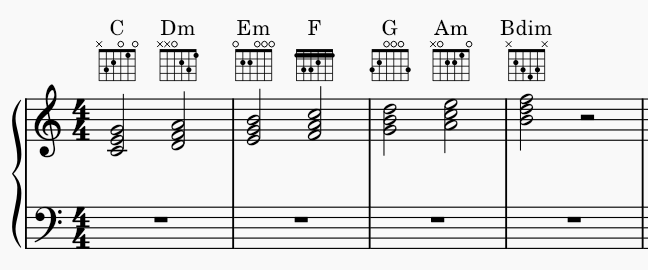
\includegraphics[width=0.5\textwidth]{img/acordes.png} 
    \end{center}
    \caption{Acordes diatonicos de la escala de do mayor}
    \label{fig:teclado_do_mayor} % Añadir una etiqueta para referencias cruzadas
\end{figure}



Estas relaciones constituyen la base de las progresiones armónicas utilizadas en gran parte de la música tonal.

Según el análisis funcional desarrollado en la teoría tonal, los acordes pueden clasificarse también por su función armónica:

\begin{figure}[h]
\centering
\[
T: I, vi \qquad S: ii, IV \qquad D: V, vii^\circ
\]
\caption{Acordes clasificados por su función armónica \cite{harrison1994harmonic}}
\end{figure}


Esta clasificación permite describir progresiones armónicas típicas como:

\begin{figure}[h]
\centering
\[
T \rightarrow S \rightarrow D \rightarrow T
\]
\caption{Progresión armonica funcional \cite{rohrmeier2011generative}}
\end{figure}

las cuales aparecen con frecuencia en la música tonal desde el período barroco hasta el romanticismo.

\subsubsection{Acordes con séptima}

La armonía tonal no se limita a tríadas. Al agregar una tercera adicional sobre una tríada se obtiene un acorde de séptima. Estos acordes introducen mayor complejidad armónica y generan tensiones que requieren resolución.

Los tipos más comunes de acordes de séptima son:

\begin{itemize}
\item Séptima mayor: $Cmaj7 = C - E - G - B$
\item Séptima dominante: $C7 = C - E - G - Bb$
\item Séptima menor: $Cm7 = C - Eb - G - Bb$
\item Séptima semidisminuida: $Cm7^{\flat5} = C - Eb - Gb - Bb$
\item Séptima disminuida: $C^\circ7 = C - Eb - Gb - Bbb$
\end{itemize}

El acorde de séptima dominante es particularmente importante en la armonía funcional porque contiene el tritono entre su tercera y su séptima, lo cual genera una fuerte tendencia a resolver hacia la tónica \cite{schoenberg1983theory}.


En la escala mayor, los acordes de séptima derivados diatónicamente son:

\begin{figure}[h]
\centering
\[
Imaj7 \quad iim7 \quad iiim7 \quad IVmaj7 \quad V7 \quad vim7 \quad vii^{\emptyset7}
\]
\caption{Acordes de diatónicos de septima \cite{levine2011jazz}}
\end{figure}

En la siguiente figura vemos la aplicación de las séptimas a la escala de do mayor:

\begin{figure}[htbp]
    \centering
    \begin{center}
        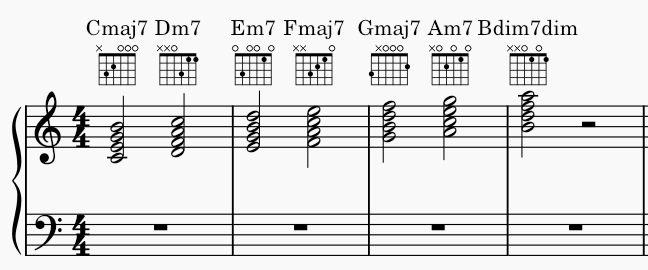
\includegraphics[width=0.5\textwidth]{img/septimas.png} 
    \end{center}
    \caption{Acordes diatonicos de septima en la escala de do mayor}
    \label{fig:teclado_do_mayor} % Añadir una etiqueta para referencias cruzadas
\end{figure}


donde $^{\emptyset7}$ indica un acorde semidisminuido.

Estos acordes amplían las posibilidades de progresión armónica y permiten describir fenómenos característicos del jazz, la música clásica tardía y diversos estilos contemporáneos.

\subsubsection{Tensiones: 9, 11 y 13}

Una extensión natural de los acordes de séptima consiste en añadir intervalos adicionales dentro de la misma estructura de terceras superpuestas. Estas extensiones se denominan tensiones y corresponden a los intervalos novena, oncena y trecena respecto a la fundamental.

Matemáticamente, estas tensiones equivalen a las siguientes notas dentro de la escala:

\begin{figure}[h]
\centering
\[
9 = 2^\mathrm{a} \qquad
11 = 4^\mathrm{a} \qquad
13 = 6^\mathrm{a}
\]

\caption{Equivalencias de tensiones \cite{russell2001lydian}}
\end{figure}

pero se consideran extensiones porque se sitúan una octava por encima \cite{terhardt1982pyschoacoustic}.

Por ejemplo:

\begin{figure}[h]
\centering
\[
C9 = C - E - G - Bb - D
\]

\[
C11 = C - E - G - Bb - D - F
\]

\[
C13 = C - E - G - Bb - D - F - A
\]

\caption{Patrón de tensiones del acorde de do mayor}
\end{figure}

Estas tensiones enriquecen la sonoridad armónica y son particularmente relevantes en estilos como el jazz y la música contemporánea.

El estudio geométrico de estas estructuras armónicas ha sido desarrollado en trabajos contemporáneos como los de Tymoczko \cite{tymoczko2006geometry}, quien propone modelos espaciales para representar las relaciones entre acordes y progresiones armónicas.

\subsubsection{Contrapunto}

En el contexto de la composición musical simbólica [cite: 52], el contrapunto se define como la interdependencia de voces melódicas regidas por una sintaxis lógica[cite: 52]. Para esta investigación, el \textit{Cantus Firmus} ($CF$) actúa como el vector de entrada base, mientras que las cuatro especies de contrapunto funcionan como el conjunto de restricciones ($\mathcal{R}$) del sistema \cite{schottstaedt1989automatic}.

\textbf{El Cantus Firmus} $CF$ es una melodía preexistente de notas de larga duración que sirve como eje estructural. En la \textbf{Representación Matricial Relativa} propuesta, cada nota $n \in CF$ se codifica no como un valor absoluto, sino como un vector que contiene su función tonal y relación interválica.


\begin{figure}[htbp]
    \centering
    \begin{center}
        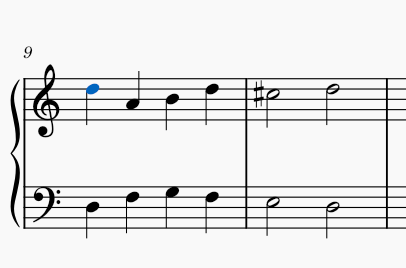
\includegraphics[width=0.5\textwidth]{img/contrapunto.png} 
    \end{center}
    \caption{Ejemplo de contrapunto de primera especie}
    \label{fig:teclado_do_mayor} % Añadir una etiqueta para referencias cruzadas
\end{figure}



A continuación se define cada una de las cuatro especies de contrapunto \cite{westergaard1975introduction}:

\begin{enumerate}
    \item \textbf{Primera Especie (Nota contra nota):} Establece una relación $1:1$ entre el $CF$ y la voz generada. 
    \begin{itemize}
        \item \textbf{Regla:} Solo se permiten intervalos de consonancia perfecta (unísono, $5^{a}$, $8^{a}$) e imperfecta ($3^{a}$, $6^{a}$).
    \end{itemize}

    \item \textbf{Segunda Especie (Dos contra una):} Introduce una relación rítmica de $2:1$. 
    \begin{itemize}
        \item \textbf{Regla:} El primer tiempo (fuerte) debe ser consonante; el segundo tiempo (débil) puede ser una \textit{nota de paso} disonante si se mueve por grado conjunto.
    \end{itemize}

    \item \textbf{Tercera Especie (Cuatro contra una):} Relación de $4:1$, permitiendo mayor varianza melódica.
    \begin{itemize}
        \item \textbf{Regla:} Permite figuras como la \textit{cambiata} o bordaduras, siempre que las disonancias no ocurran en los acentos métricos principales.
    \end{itemize}

    \item \textbf{Cuarta Especie (Síncopas):} Utiliza suspensiones para generar tensión y resolución.
    \begin{itemize}
        \item \textbf{Regla:} Una nota consonante se prolonga hacia el siguiente compás convirtiéndose en disonancia (suspensión), la cual \textbf{debe} resolver descendentemente por grado conjunto.
     \end{itemize}
\end{enumerate}


\subsubsection{Modos griegos o modos eclesiásticos medievales}

Antes de la consolidación del sistema tonal mayor-menor, la música occidental utilizaba diversos sistemas modales. Los llamados modos griegos —o más propiamente modos eclesiásticos medievales— representan diferentes configuraciones de intervalos dentro de la escala diatónica.

Los siete modos principales derivados de la escala mayor son: Jónico, Dórico, Frigio, Lidio,Mixolidio, Eólico y Locrio.


Cada modo puede entenderse como una rotación de la escala mayor \cite{carey1989aspects}. Por ejemplo:
\begin{figure}[h]
\centering
\[
\begin{aligned}
\text{Jónico:}      &\; C\; D\; E\; F\; G\; A\; B \\
\text{Dórico:}      &\; D\; E\; F\; G\; A\; B\; C \\
\text{Frigio:}      &\; E\; F\; G\; A\; B\; C\; D \\
\text{Lidio:}       &\; F\; G\; A\; B\; C\; D\; E \\
\text{Mixolidio:}   &\; G\; A\; B\; C\; D\; E\; F \\
\text{Eólico:}      &\; A\; B\; C\; D\; E\; F\; G \\
\text{Locrio:}      &\; B\; C\; D\; E\; F\; G\; A
\end{aligned}
\]
\caption{Modos griegos o modos eclesiásticos medievales}
\end{figure}

Cada modo posee un carácter sonoro particular debido a la disposición de tonos y semitonos.

Los modos desempeñaron un papel central en la música medieval y renacentista, y han sido retomados en contextos modernos como el jazz modal y la música contemporánea. Desde una perspectiva analítica, pueden interpretarse como diferentes regiones dentro del espacio armónico descrito por Tymoczko, donde las transformaciones entre acordes y escalas pueden representarse mediante geometrías musicales.

Asimismo, el estudio de la armonía funcional fue profundamente reformulado en el siglo XX por Arnold Schoenberg, quien analizó la tonalidad como un sistema de fuerzas dirigidas y tensiones estructurales. Sus tratados influyeron significativamente en la teoría musical moderna y en la comprensión de la transición hacia lenguajes armónicos más complejos \cite{brent2011modalogy}.

\subsubsection{Conclusión}

La armonía funcional, el contrapunto y los sistemas modales representan tres enfoques complementarios para comprender la organización musical. Mientras que la armonía funcional describe las relaciones jerárquicas entre acordes dentro de una tonalidad, el contrapunto analiza la interacción entre voces independientes y los modos ofrecen sistemas alternativos de organización de las alturas. Estos marcos conceptuales han evolucionado a lo largo de siglos de práctica musical y continúan siendo herramientas fundamentales tanto para la composición como para el análisis teórico \cite{pachet1998content}.

\subsection{Espacios geométricos musicales y conducción de voces}
Una de las aproximaciones contemporáneas más influyentes para el estudio de la armonía y la conducción de voces consiste en modelar las relaciones entre acordes y estructuras musicales mediante espacios geométricos. Este enfoque parte de la idea de que las configuraciones de alturas musicales pueden representarse como puntos dentro de un espacio matemático, donde las distancias reflejan transformaciones musicales como el movimiento de voces o la relación entre acordes. A través de esta perspectiva, fenómenos tradicionalmente descritos mediante reglas armónicas pueden analizarse utilizando herramientas de la geometría, la topología y la teoría de grupos \cite{roeder1984geometric}.

En la teoría musical tradicional, la conducción de voces describe la manera en que las diferentes voces de una textura polifónica se desplazan de un acorde a otro. Este concepto es fundamental en el análisis de la música tonal, especialmente en la práctica común de los siglos XVII al XIX. Las reglas de conducción de voces buscan minimizar movimientos innecesarios entre las notas de los acordes, favorecer el movimiento conjunto y evitar paralelismos considerados problemáticos, como quintas u octavas paralelas. En términos generales, la conducción de voces eficiente implica que las notas individuales se muevan lo menos posible al pasar de una sonoridad a otra \cite{tymoczko2006geometry7274}.

El enfoque geométrico formaliza esta intuición mediante la representación de los acordes como puntos en un espacio multidimensional. Si consideramos un acorde compuesto por $n$ notas, cada nota puede representarse como una coordenada que corresponde a su altura en una escala cromática. De esta manera, un acorde puede representarse como un vector \cite{callender2008generalized}:

\begin{figure}[h]
\centering
\[
(x_1, x_2, \dots, x_n)
\]
\caption{Representación de acordes como puntos}
\end{figure}


donde cada $x_i$ representa la altura de una voz específica. La transición entre dos acordes puede interpretarse entonces como el desplazamiento entre dos puntos en este espacio. La distancia entre dichos puntos representa la cantidad total de movimiento requerido por las voces.

Sin embargo, la música presenta ciertas simetrías que deben tenerse en cuenta al construir estos espacios. Por ejemplo, las octavas se perciben como equivalentes en muchos contextos musicales, lo que significa que dos notas separadas por una octava pueden considerarse funcionalmente iguales dentro de ciertos modelos. Asimismo, el orden de las voces puede ser irrelevante cuando se estudian únicamente las clases de acordes. Estas consideraciones conducen a la construcción de espacios geométricos más sofisticados donde se identifican puntos equivalentes mediante relaciones de simetría.

En su trabajo sobre la geometría de la música, Tymoczko\cite{tymoczko2011geometry} propone representar los acordes dentro de espacios llamados orbifolds, que surgen al considerar las equivalencias entre permutaciones de voces, transposiciones y equivalencias de octava. Estos espacios permiten visualizar las relaciones entre acordes como trayectorias continuas dentro de una estructura geométrica. En particular, las progresiones armónicas comunes corresponden a caminos cortos dentro de estos espacios, lo que refleja el principio de conducción de voces eficiente.

Por ejemplo, la transición entre los acordes $C$ mayor $(C,E,G)$ y $F$ mayor $(F,A,C)$ puede describirse como un movimiento relativamente pequeño en el espacio de acordes, ya que varias notas pueden desplazarse por intervalos cortos. En términos geométricos, esta transición corresponde a un desplazamiento corto entre dos puntos dentro del espacio tridimensional asociado a tríadas \cite{bent2011modalogy}.

Otro aspecto importante de estos modelos es la noción de distancia musical. Existen diferentes métricas que pueden utilizarse para medir la distancia entre acordes, dependiendo del tipo de transformación que se desee modelar. Una métrica común consiste en minimizar la suma de los movimientos absolutos de cada voz al pasar de un acorde a otro. Esta métrica captura formalmente la idea de que las progresiones armónicas tienden a favorecer movimientos pequeños y suaves entre las voces \cite{tymoczko2008scale}.

Los espacios geométricos también permiten describir transformaciones armónicas más complejas. Por ejemplo, ciertas progresiones características de la música romántica o del jazz pueden interpretarse como trayectorias específicas dentro de estos espacios. De manera similar, relaciones entre acordes aparentemente distantes pueden visualizarse como conexiones cercanas cuando se consideran transformaciones como la inversión o la equivalencia de octava.

El Tonnetz, originalmente introducido en el siglo XIX por teóricos como Euler y posteriormente desarrollado por Riemann \cite{cohn1997neo}, constituye uno de los antecedentes históricos más importantes de los modelos geométricos modernos. En esta red bidimensional, las notas se organizan de manera que los acordes mayores y menores aparecen como triángulos conectados. Las transformaciones entre acordes pueden representarse como desplazamientos dentro de esta red.

\begin{figure}[htbp]
    \centering
    \begin{center}
        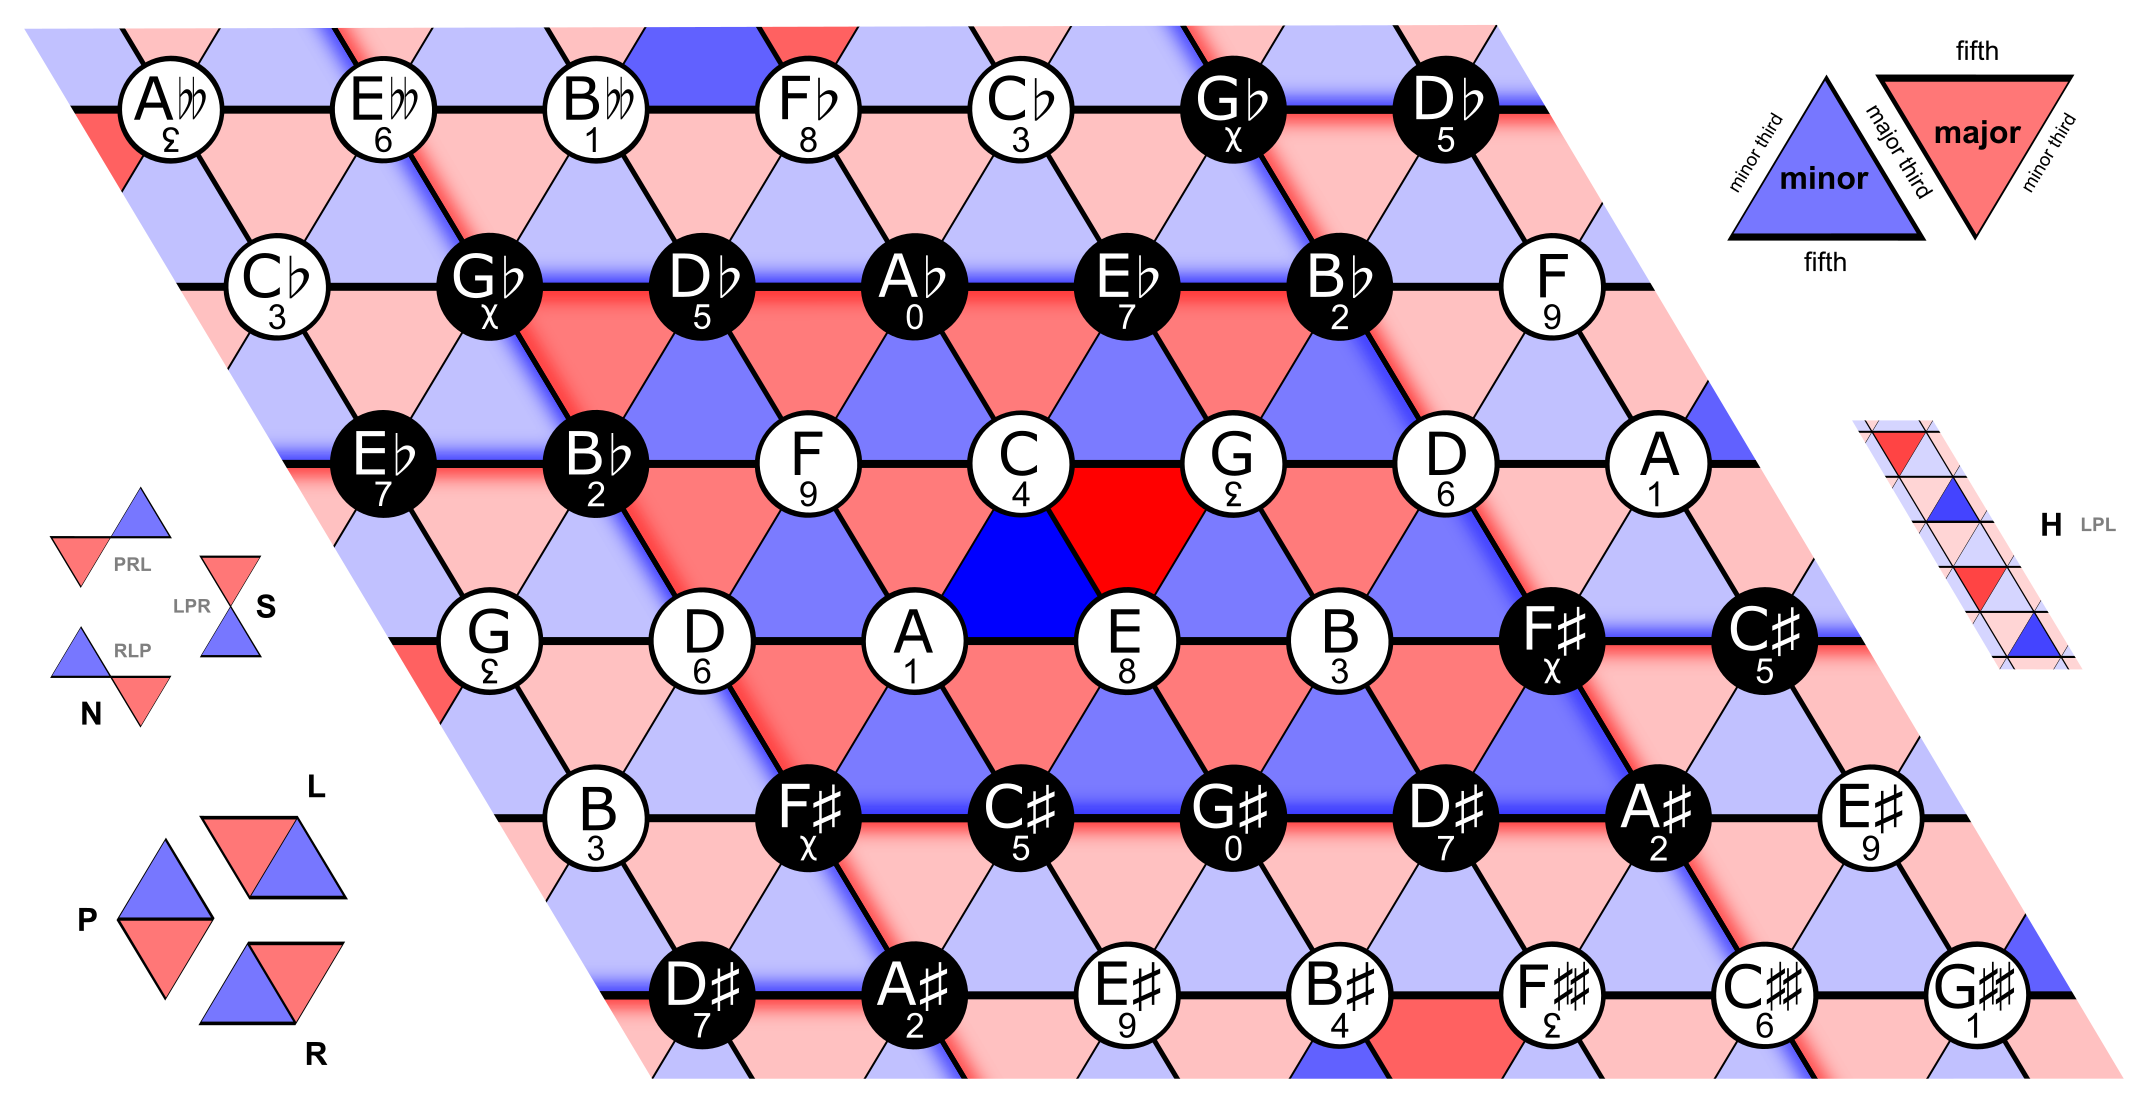
\includegraphics[width=0.5\textwidth]{img/tonnetz.png} 
    \end{center}
    \caption{Red de tonos o Tonnetz \cite{catanzaro2011topological}}
    \label{fig:teclado_do_mayor} % Añadir una etiqueta para referencias cruzadas
\end{figure}


La formalización matemática de estos conceptos ha permitido establecer conexiones entre la teoría musical y diversas áreas de las matemáticas. En particular, la topología y la geometría diferencial han sido utilizadas para describir las propiedades estructurales de los espacios de acordes. Estos modelos también han encontrado aplicaciones en campos como la musicología computacional, donde se utilizan para analizar grandes corpus musicales o para desarrollar algoritmos de generación automática de armonías \cite{bergomi2015topological}.

Además, los espacios geométricos musicales ofrecen una herramienta pedagógica poderosa, ya que permiten visualizar conceptos abstractos de la teoría musical. Al representar acordes y progresiones como puntos y trayectorias dentro de un espacio, los estudiantes pueden comprender de manera intuitiva cómo se relacionan diferentes estructuras armónicas \cite{hall2008topology}.

En conclusión, el enfoque geométrico de la música proporciona un marco unificado para analizar la conducción de voces y las relaciones armónicas. Al modelar los acordes como puntos dentro de espacios matemáticos estructurados, es posible describir de manera precisa fenómenos que tradicionalmente se explicaban mediante reglas heurísticas. Este enfoque no solo amplía nuestra comprensión teórica de la música, sino que también abre nuevas posibilidades para la investigación interdisciplinaria entre música, matemáticas y ciencias computacionales.

\section{Representación de Datos en IA Musical}
\subsection{Representaciones Absolutas vs. Relativas}
Uno de los aspectos fundamentales en el desarrollo de sistemas de inteligencia artificial aplicados a la música es la forma en que los datos musicales son representados para su procesamiento computacional. La música, en su forma acústica, es una señal continua en el tiempo; sin embargo, para poder ser analizada o generada por algoritmos, debe transformarse en estructuras discretas y manipulables. Dentro de este contexto, existen dos enfoques principales para representar información musical: las representaciones absolutas y las representaciones relativas. Cada una de estas aproximaciones tiene implicaciones distintas en términos de generalización, aprendizaje estadístico y capacidad de modelado de estructuras musicales.

Las representaciones absolutas describen los eventos musicales utilizando valores específicos de altura, duración o tiempo sin considerar explícitamente las relaciones estructurales entre ellos. En este enfoque, cada nota se representa mediante atributos concretos, como su número MIDI \cite{midi1996specification}, su duración en unidades temporales discretas o su posición dentro de una secuencia. Por ejemplo, en el estándar MIDI, las alturas se representan mediante enteros entre 0 y 127, donde cada número corresponde a una frecuencia específica dentro del sistema de temperamento igual. De esta manera, una melodía puede representarse como una secuencia de números que indican las alturas absolutas de las notas \cite{briot2020deep}.

Una forma común de representación absoluta consiste en el uso de matrices que codifican eventos musicales en función del tiempo y la altura. En este esquema, las filas de la matriz corresponden a diferentes alturas o clases de notas, mientras que las columnas representan unidades discretas de tiempo. Un valor binario o real dentro de la matriz indica la presencia o intensidad de una nota en un momento determinado. Este tipo de representación, conocido frecuentemente como \textit{piano roll}, es ampliamente utilizado en sistemas de aprendizaje automático para música simbólica.

\begin{figure}[htbp]
    \centering
    \begin{center}
        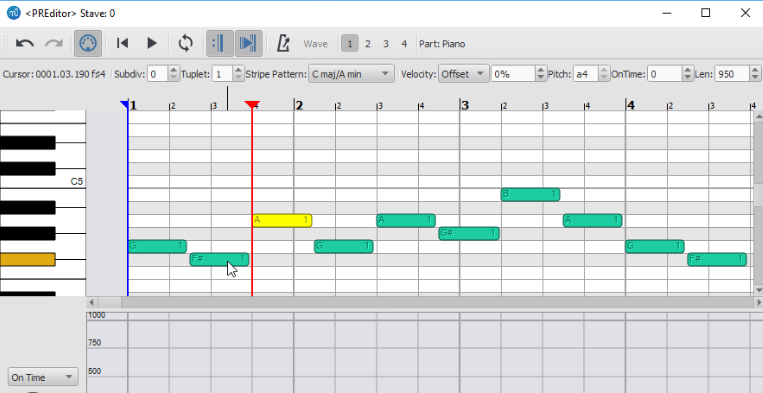
\includegraphics[width=0.5\textwidth]{img/pianoroll.png} 
    \end{center}
    \caption{Interfaz de piano roll \cite{dong2018musegan}}
    \label{fig:teclado_do_mayor} % Añadir una etiqueta para referencias cruzadas
\end{figure}


Formalmente, una representación matricial absoluta puede describirse como
\begin{figure}[h]
\centering
\[
X \in \mathbb{R}^{P \times T}
\]
\caption{Representación absoluta}
\end{figure}


donde $P$ representa el número de posibles alturas (por ejemplo, 128 valores MIDI) y $T$ el número de pasos temporales discretizados. Cada elemento $X_{p,t}$ indica la presencia o intensidad de la altura $p$ en el instante $t$.

Las representaciones absolutas tienen la ventaja de ser simples y directas, lo que facilita su integración con modelos de aprendizaje profundo como redes neuronales recurrentes, redes convolucionales o transformadores. Sin embargo, presentan ciertas limitaciones cuando se trata de capturar relaciones musicales abstractas. Por ejemplo, dos melodías idénticas pero transpuestas a diferentes tonalidades se representan como secuencias completamente distintas en términos absolutos, lo que puede dificultar la generalización del modelo \cite{huang2018music}.

Para abordar este problema, se utilizan representaciones relativas, las cuales describen la música en términos de relaciones entre eventos musicales en lugar de valores absolutos. En este enfoque, las alturas no se codifican directamente, sino que se representan mediante intervalos respecto a una nota anterior o a un centro tonal. Por ejemplo, en lugar de representar una melodía como la secuencia de alturas

\begin{figure}[h]
\centering
\[
[60, 62, 64, 65, 67]
\]
\caption{Ejemplo de representación absoluta}
\end{figure}


una representación relativa podría codificarla como una secuencia de intervalos

\begin{figure}[h]
\centering
\[
[+2, +2, +1, +2]
\]
\caption{Ejemplo de representación relativa}
\end{figure}


que describen los desplazamientos entre notas consecutivas \cite{conklin1995multiple}.

Este tipo de representación refleja de manera más directa ciertos principios fundamentales de la teoría musical, donde las relaciones intervalares y las estructuras tonales desempeñan un papel central. Además, las representaciones relativas permiten capturar invariancias musicales importantes, como la equivalencia entre melodías transpuestas a diferentes tonalidades.

Otra forma de representación relativa consiste en describir las notas en función de su posición dentro de una escala o de un acorde. Por ejemplo, una melodía puede codificarse mediante grados de la escala en lugar de alturas absolutas. De esta manera, el patrón melódico se mantiene constante incluso cuando cambia la tonalidad. Este enfoque resulta particularmente útil en tareas como la generación automática de melodías o el análisis de progresiones armónicas \cite{temperley2004bayesian}.

Las representaciones relativas también se han utilizado en modelos modernos de aprendizaje profundo para capturar dependencias musicales de largo alcance. En particular, ciertos modelos basados en arquitecturas de transformadores utilizan mecanismos de atención relativa que codifican la distancia entre eventos musicales en lugar de sus posiciones absolutas. Este enfoque permite modelar estructuras musicales como repeticiones, secuencias y patrones rítmicos de manera más eficiente \cite{shaw2018self}.



Desde una perspectiva computacional, la elección entre representaciones absolutas y relativas depende en gran medida del tipo de tarea que se desea abordar. Las representaciones absolutas suelen ser adecuadas para tareas donde la información precisa de altura y tiempo es esencial, como la síntesis musical o la transcripción automática de audio a notación. En cambio, las representaciones relativas resultan particularmente útiles para tareas que requieren capturar patrones estructurales, como la generación de melodías, el análisis estilístico o la modelización de progresiones armónicas \cite{roberts2018hierarchical}.

En muchos sistemas modernos de inteligencia artificial musical se utilizan enfoques híbridos que combinan ambos tipos de representación. Por ejemplo, un modelo puede utilizar alturas absolutas para describir eventos musicales concretos mientras emplea codificaciones relativas para capturar relaciones estructurales entre ellos. Esta combinación permite aprovechar las ventajas de ambas aproximaciones y mejorar la capacidad de generalización del modelo \cite{wiering2009modeling}.

En conclusión, la representación de datos constituye un elemento crucial en el diseño de sistemas de inteligencia artificial musical. Las representaciones absolutas ofrecen una descripción directa y detallada de los eventos musicales, mientras que las representaciones relativas permiten capturar relaciones estructurales e invariancias fundamentales del lenguaje musical. La elección adecuada entre estos enfoques —o la combinación de ambos— puede influir significativamente en el rendimiento y la capacidad de aprendizaje de los modelos computacionales aplicados al análisis y generación de música.

\subsection{El concepto de Representación Matricial Relativa de Armonía Funcional}
En los sistemas de inteligencia artificial aplicados a la música, la forma en que se codifica la información armónica tiene un impacto significativo en la capacidad del modelo para aprender patrones musicales. Mientras que muchas representaciones tradicionales utilizan codificaciones absolutas de acordes o alturas, en numerosos contextos resulta más adecuado emplear representaciones relativas que capturen las relaciones funcionales entre los elementos armónicos. En este contexto surge el concepto de representación matricial relativa de la armonía funcional, una estrategia de codificación que describe progresiones armónicas en función de sus relaciones dentro de una tonalidad en lugar de sus valores absolutos de altura \cite{hadjeres2017deepbach}.

La armonía funcional, como se discutió en secciones anteriores, describe los acordes en términos de su papel dentro de una escala tonal. En lugar de tratar los acordes como colecciones independientes de notas, se clasifican según su función armónica, como tónica, subdominante o dominante. Esta organización permite identificar regularidades estructurales en la música tonal que se mantienen invariantes bajo transformaciones como la transposición. Por ejemplo, la progresión armónica I–IV–V–I conserva su estructura funcional independientemente de la tonalidad en la que se interprete \cite{dehaas2013modeling}.

En una representación absoluta, esta progresión podría aparecer como:

\begin{figure}[h]
\centering
\[
C \quad F \quad G \quad C
\]
\caption{Progresión absoluta}
\end{figure}


en la tonalidad de Do mayor, o como

\begin{figure}[h]
\centering
\[
D \quad G \quad A \quad D
\]
\caption{Progresión absoluta en re mayor}
\end{figure}



en la tonalidad de Re mayor. Aunque ambas secuencias cumplen la misma función armónica, sus representaciones absolutas difieren completamente en términos de alturas. Esto puede dificultar el aprendizaje de patrones armónicos generales por parte de un modelo de aprendizaje automático.

La representación matricial relativa resuelve este problema codificando los acordes según su grado dentro de la escala o su función tonal. En este caso, ambas progresiones se representarían simplemente como:

\begin{figure}[h]
\centering
\[
I \quad IV \quad V \quad I
\]
\caption{Representación realativa de las progresiones}
\end{figure}


De esta manera, el modelo puede aprender la estructura armónica sin depender de una tonalidad específica \cite{collins2014computational}.

Para su implementación computacional, estas representaciones suelen organizarse en matrices que describen la presencia o transición entre grados armónicos a lo largo del tiempo. Una posible formulación consiste en representar una secuencia armónica mediante una matriz

\begin{figure}[h]
\centering
\[
H \in \mathbb{R}^{G \times T}
\]
\caption{Representación computacional realativa de las progresiones \cite{christensen2002cambridge}}
\end{figure}


donde $G$ representa el número de posibles grados armónicos dentro del sistema tonal y $T$ el número de pasos temporales discretos. Cada elemento $H_{g,t}$ indica la presencia o probabilidad de que el grado armónico $g$ ocurra en el instante temporal $t$.

Otra variante de esta representación consiste en utilizar matrices de transición armónica, en las cuales cada entrada describe la probabilidad de transición entre dos grados funcionales. Estas matrices pueden interpretarse como grafos dirigidos donde los nodos representan funciones armónicas y las aristas representan movimientos entre ellas. Este tipo de estructura ha sido utilizado ampliamente en modelos probabilísticos de música, como las cadenas de Markov aplicadas al análisis y generación de progresiones armónicas \cite{pachet2011finite}. 

\begin{figure}[htbp]
    \centering
    \begin{center}
        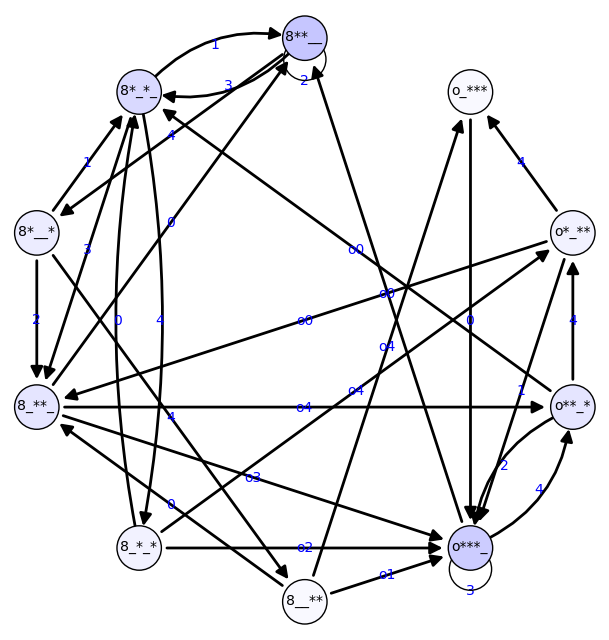
\includegraphics[width=0.5\textwidth]{img/grafos.png} 
    \end{center}
    \caption{Respresentación visual de un grafo}
    \label{fig:teclado_do_mayor} % Añadir una etiqueta para referencias cruzadas
\end{figure}

Además de facilitar el aprendizaje estadístico, las representaciones relativas presentan ventajas importantes desde el punto de vista musical. Al codificar las progresiones en términos de funciones tonales, se preservan propiedades estructurales fundamentales del lenguaje armónico, como las relaciones de tensión y resolución entre dominante y tónica. Asimismo, esta representación permite integrar conocimientos teóricos de la armonía dentro de modelos computacionales, lo cual puede mejorar la interpretabilidad de los resultados generados por sistemas de inteligencia artificial \cite{farbood2012quantifying}.

En modelos más avanzados, las representaciones matriciales relativas pueden combinarse con información adicional como inversiones de acordes, tensiones armónicas o contextos modales. Esto permite capturar niveles más profundos de la estructura armónica sin perder las ventajas de la invariancia tonal. De igual manera, algunos enfoques incorporan información sobre conducción de voces o proximidad armónica dentro de espacios geométricos musicales, integrando así distintas dimensiones de la teoría musical en una representación computacional coherente.

En conclusión, la representación matricial relativa de la armonía funcional constituye una herramienta poderosa para modelar progresiones armónicas en sistemas de inteligencia artificial musical. Al abstraer las relaciones armónicas fundamentales y eliminar la dependencia de tonalidades específicas, este enfoque facilita el aprendizaje de patrones musicales generales y mejora la capacidad de los modelos para generar o analizar música dentro de diferentes contextos tonales.


\section{Inteligencia artíficial para la generación musical}

\subsection{Redes neuronales como generadores musicales estocasticos}
Las redes neuronales profundas han demostrado ser una de las herramientas más eficaces para modelar datos secuenciales complejos. En el contexto de la inteligencia artificial musical, estas arquitecturas permiten aprender patrones temporales presentes en melodías, progresiones armónicas y estructuras rítmicas. En particular, las redes neuronales recurrentes (RNN, por sus siglas en inglés) se han utilizado ampliamente para la generación estocástica de música debido a su capacidad para modelar dependencias temporales entre eventos musicales consecutivos \cite{todd1989connectionist}.

La arquitectura del modelo se fundamenta en la composición de capas neuronales, donde cada una actúa como una función paramétrica que transforma las representaciones del nivel anterior. Formalmente, la activación de una capa intermedia $l$ se define mediante la siguiente expresión:

\begin{figure}[h]
    \centering
    \[
    \mathbf{h}^{(l)} = \sigma \left( \mathbf{W}^{(l)} \mathbf{h}^{(l-1)} + \mathbf{b}^{(l)} \right)
    \]
    \caption{Representación matemática de una capa neuronal funcional. \cite{goodfellow2016deep}}
    \label{fig:neural_layer}
\end{figure}

Donde:
\begin{itemize}
    \item $\mathbf{h}^{(l)} \in \mathbb{R}^{d_l}$ representa el vector de activación (o estado oculto) de la capa $l$.
    \item $\mathbf{W}^{(l)} \in \mathbb{R}^{d_l \times d_{l-1}}$ es la matriz de pesos sinápticos que conecta la capa $l-1$ con la capa $l$.
    \item $\mathbf{b}^{(l)} \in \mathbb{R}^{d_l}$ es el vector de sesgo (\textit{bias}) que permite el desplazamiento de la función de activación.
    \item $\sigma(\cdot)$ denota la función de activación no lineal (e.g., \textit{ReLU, Sigmoid} o \textit{Tanh}), la cual dota a la red de la capacidad de aproximar funciones no lineales complejas.
\end{itemize}

Una red neuronal puede entenderse como una función paramétrica compuesta por múltiples capas que transforman una entrada en una salida mediante operaciones lineales y funciones de activación no lineales. En términos generales, una capa neuronal realiza una transformación de la forma

\begin{figure}[htbp]
    \centering
    \begin{equation}
        \mathbf{h} = \sigma(\mathbf{W}\mathbf{x} + \mathbf{b})
        \label{eq:capa_neuronal}
    \end{equation}
    \caption{Función de transformación lineal y activación en una capa densa \cite{lecun2015deep}.}
\end{figure}



donde $x$ representa el vector de entrada, $W$ es la matriz de pesos, $b$ es un vector de sesgos y $\sigma$ corresponde a una función de activación no lineal. La composición de múltiples capas permite construir representaciones jerárquicas cada vez más abstractas de los datos de entrada.

Sin embargo, las redes neuronales tradicionales o \textit{feedforward} \cite{rumelhart1986learning} presentan limitaciones cuando se aplican a datos secuenciales, ya que procesan cada entrada de forma independiente. En contraste, las redes neuronales recurrentes incorporan un estado interno que se actualiza a lo largo del tiempo, permitiendo que la red mantenga memoria de eventos anteriores dentro de la secuencia.

Formalmente, una red neuronal puede describirse mediante la ecuación recursiva

\begin{figure}[htbp]
    \centering
    \begin{equation}
        \mathbf{h}_t = \sigma(\mathbf{W}_x \mathbf{x}_t + \mathbf{W}_h \mathbf{h}_{t-1} + \mathbf{b})
        \label{eq:rnn_recursiva}
    \end{equation}
    \caption{Representación matemática de la actualización del estado oculto en una Red Neuronal Recurrente (RNN).}
\end{figure}

donde $x_t$ representa la entrada en el tiempo $t$, $h_t$ es el estado oculto de la red y $h_{t-1}$ corresponde al estado del paso temporal anterior. Esta estructura permite que la red capture dependencias temporales dentro de secuencias musicales, como patrones rítmicos recurrentes o relaciones melódicas entre notas consecutivas.

En el presente proyecto, las redes neuronales se implementarán utilizando la biblioteca TensorFlow, una de las plataformas más utilizadas para el desarrollo de modelos de aprendizaje profundo. TensorFlow proporciona herramientas de alto nivel para definir arquitecturas neuronales complejas, entrenarlas mediante optimización basada en gradiente y desplegarlas en distintos entornos computacionales. En particular, la interfaz Keras integrada en TensorFlow facilita la construcción modular de redes neuronales mediante la composición de capas \cite{abadi2016tensorflow}.

Dado que el objetivo del sistema es explorar diferentes arquitecturas dentro de un marco evolutivo, se experimentará con múltiples tipos de capas neuronales. Entre las más relevantes se encuentran las capas densas (\textit{Dense}), que realizan transformaciones completamente conectadas; las capas recurrentes simples (\textit{SimpleRNN}); y variantes más avanzadas como las capas LSTM (\textit{Long Short-Term Memory}) y GRU (\textit{Gated Recurrent Units}). Estas últimas introducen mecanismos de compuertas que permiten controlar el flujo de información dentro de la red, mitigando problemas clásicos de las RNN como el desvanecimiento del gradiente \cite{bengio1994learning}.

Las capas LSTM, por ejemplo, incorporan estructuras internas que regulan qué información debe almacenarse, actualizarse o descartarse a lo largo del tiempo. Estas compuertas permiten que la red mantenga información relevante durante intervalos temporales más largos, lo cual resulta particularmente útil en tareas musicales donde ciertos patrones pueden repetirse después de varios compases \cite{eck2002finding}.

La salida de la red neuronal se interpretará como una distribución de probabilidad sobre posibles eventos musicales. En lugar de seleccionar determinísticamente el evento con mayor probabilidad, el sistema utilizará muestreo estocástico para generar nuevas secuencias musicales. Este enfoque permite introducir variabilidad creativa en las composiciones generadas y evita que el modelo produzca siempre las mismas secuencias \cite{holtzman2019curious}.

Si denotamos la salida de la red en el instante $t$ como un vector de probabilidades


\begin{figure}[htbp]
    \centering
    \begin{equation}
        \mathbf{p}_t = (p_{t,1}, p_{t,2}, \dots, p_{t,n})
        \label{eq:vector_probabilidades}
    \end{equation}
    \caption{Representación del vector de probabilidades de salida $\mathbf{p}_t$ en el instante discreto $t$.}
\end{figure}

donde cada componente $p_i$ representa la probabilidad de seleccionar un evento musical específico, entonces la generación estocástica consiste en muestrear un evento según dicha distribución. Este procedimiento se utiliza ampliamente en modelos generativos modernos y permite equilibrar coherencia estructural con diversidad creativa.

Durante el proceso de entrenamiento, la red se optimiza utilizando algoritmos de descenso de gradiente, como Adam \cite{kingma2014adam} o RMSProp. Estos métodos ajustan los parámetros del modelo para minimizar una función de pérdida que mide la diferencia entre las predicciones de la red y los datos reales del conjunto de entrenamiento. En el caso de modelos generativos de secuencias, es común utilizar la entropía cruzada como función de pérdida, ya que permite comparar distribuciones de probabilidad.

Un aspecto importante del presente sistema es que la arquitectura exacta de la red neuronal no se definirá de manera fija. En cambio, como se discutió en secciones anteriores, un algoritmo genético \cite{stanley2002evolving} explorará diferentes configuraciones posibles de capas y parámetros. Esto incluye variaciones en el número de capas recurrentes, el tamaño de los estados ocultos, los tipos de funciones de activación y otros hiperparámetros relevantes. De esta manera, el sistema podrá descubrir arquitecturas particularmente adecuadas para modelar estructuras musicales específicas.

La integración de redes neuronales recurrentes dentro de una arquitectura híbrida que también incluye sistemas evolutivos y filtros basados en reglas permite combinar diferentes paradigmas de inteligencia artificial \cite{miranda2013evolutionary}. Mientras que las RNN capturan regularidades estadísticas complejas presentes en los datos musicales, los componentes evolutivos exploran configuraciones arquitectónicas y los sistemas basados en reglas garantizan el cumplimiento de restricciones teóricas. Esta combinación proporciona un marco robusto para el desarrollo de sistemas de generación musical asistidos por inteligencia artificial .

En conclusión, las redes neuronales recurrentes implementadas en TensorFlow constituyen el núcleo generativo del sistema propuesto. Su capacidad para modelar dependencias temporales y producir secuencias estocásticas las convierte en herramientas especialmente adecuadas para la generación musical. Al combinar estas arquitecturas con métodos evolutivos y filtros basados en reglas, el sistema busca aprovechar las fortalezas de distintos enfoques de inteligencia artificial para producir resultados musicalmente coherentes y estilísticamente variados.

\subsection{Árboles de Decisión como filtros de restricción armónica}
En los sistemas contemporáneos de generación musical basados en aprendizaje automático, uno de los principales desafíos consiste en equilibrar la capacidad creativa de los modelos generativos con el cumplimiento de reglas estructurales propias del lenguaje musical. Las redes neuronales profundas son particularmente eficaces para aprender patrones estadísticos a partir de grandes conjuntos de datos, pero no siempre garantizan que las salidas generadas respeten restricciones teóricas específicas \cite{briot2020deep}, como las reglas de la armonía tonal o del contrapunto. Para abordar este problema, es posible integrar sistemas basados en reglas dentro de la arquitectura general del modelo. En el presente proyecto, los árboles de decisión se utilizarán como mecanismos de filtrado para aplicar restricciones armónicas estrictas, conocidas como \textit{hard constraints}, sobre las secuencias musicales generadas por la red neuronal.

Los árboles de decisión constituyen una clase de modelos de aprendizaje supervisado ampliamente utilizados en tareas de clasificación y regresión. Su estructura consiste en una representación jerárquica de decisiones donde cada nodo interno corresponde a una prueba lógica sobre alguna característica de los datos, y cada rama representa el resultado posible de dicha prueba. Las hojas del árbol contienen la decisión final o la categoría asignada \cite{breiman2017classification}. Una de las principales ventajas de los árboles de decisión es su interpretabilidad, ya que el proceso de inferencia puede describirse mediante una secuencia explícita de reglas condicionales \cite{molnar2020interpretable}.

En el contexto de este sistema híbrido de generación musical, los árboles de decisión no se utilizarán como modelos predictivos tradicionales, sino como filtros estructurales aplicados sobre la salida generada por la red neuronal. Específicamente, después de que la red produzca una secuencia de notas o acordes candidatos, el árbol de decisión evaluará dicha secuencia para verificar si cumple con un conjunto de restricciones armónicas previamente definidas. Si la secuencia viola alguna de estas reglas, el sistema puede rechazarla, modificarla o solicitar una nueva generación al modelo neuronal \cite{pachet2011finite}.

Este enfoque permite combinar la flexibilidad estadística de las redes neuronales con la precisión normativa de los sistemas basados en reglas. En lugar de exigir que la red neuronal aprenda explícitamente todas las restricciones teóricas del lenguaje musical, el modelo puede concentrarse en capturar patrones estilísticos generales, mientras que el árbol de decisión garantiza que el resultado final permanezca dentro de un espacio musicalmente válido \cite{papadopoulos1999ai}.

Las restricciones aplicadas por el árbol de decisión pueden definirse en función de diversos parámetros del sistema. Uno de los parámetros fundamentales es la tonalidad. En la música tonal, cada pieza se organiza alrededor de un centro tonal específico, lo que implica que las notas y acordes utilizados deben pertenecer, en general, a la escala correspondiente. El árbol de decisión puede verificar si las notas generadas pertenecen al conjunto permitido de alturas dentro de la tonalidad seleccionada. En caso contrario, el sistema puede aplicar correcciones automáticas o descartar la secuencia \cite{lerdahl1985generative}.

Otro parámetro relevante es el modo musical. Como se discutió en secciones anteriores, los modos definen diferentes configuraciones intervalares dentro de una escala diatónica. Dependiendo del modo seleccionado (por ejemplo, jónico, dórico o mixolidio), ciertas alturas pueden ser preferidas o restringidas. El árbol de decisión puede incorporar reglas específicas para cada modo, evaluando si las progresiones generadas respetan estas configuraciones modales.

Además de las restricciones tonales y modales, el sistema puede incorporar reglas derivadas del contrapunto clásico. Estas reglas regulan la conducción de voces y buscan evitar configuraciones consideradas problemáticas dentro de la tradición polifónica occidental. Entre las restricciones más comunes se encuentran la prohibición de quintas y octavas paralelas, la preferencia por el movimiento contrario entre voces y el tratamiento adecuado de disonancias \cite{fux1965study}. En este contexto, cada nodo del árbol de decisión puede evaluar condiciones específicas relacionadas con la relación entre notas consecutivas o simultáneas dentro de la textura musical.

Formalmente, el proceso de filtrado puede describirse como una función de validación aplicada a la salida del modelo neuronal. Si denotamos la secuencia generada por la red como
\begin{figure}[h]
\centering
\[
S = (s_1, s_2, \dots, s_T)
\]
\caption{Salida de la red neuronal}
\end{figure}


donde cada $s_t$ representa un evento musical en el instante $t$, el árbol de decisión implementa una función

\begin{figure}[h]
\centering
\[
f(S) \rightarrow \{0,1\}
\]
\caption{Función del arbol de decisión}
\end{figure}


donde el valor $1$ indica que la secuencia cumple con todas las restricciones armónicas establecidas, mientras que el valor $0$ indica que la secuencia debe ser descartada o corregida \cite{herremans2017morpheus}.

Este mecanismo de filtrado puede integrarse dentro de un ciclo iterativo de generación. En cada iteración, la red neuronal produce una nueva secuencia candidata, la cual es evaluada por el árbol de decisión. Si la secuencia no cumple las restricciones, el sistema genera una alternativa hasta encontrar una solución válida. Este proceso puede interpretarse como una forma de búsqueda guiada dentro del espacio de posibles secuencias musicales \cite{hadjeres2017deepbach}.

Una ventaja adicional de este enfoque es su modularidad. Las reglas implementadas en el árbol de decisión pueden modificarse fácilmente para adaptarse a diferentes estilos musicales o niveles de complejidad teórica. Por ejemplo, un modo de operación básico podría aplicar únicamente restricciones tonales, mientras que un modo avanzado podría incluir reglas detalladas de contrapunto y conducción de voces.

En conjunto, la incorporación de árboles de decisión como filtros de restricciones armónicas permite construir una arquitectura híbrida donde los modelos generativos y los sistemas simbólicos trabajan de manera complementaria. Mientras que la red neuronal explora el espacio creativo de posibles secuencias musicales, el sistema basado en reglas garantiza que los resultados finales respeten principios fundamentales de la teoría musical. Este tipo de integración entre aprendizaje automático y conocimiento experto representa una dirección prometedora para el desarrollo de sistemas de inteligencia artificial musical más robustos, interpretables y musicalmente coherentes \cite{garcez2020neurosymbolic}.


\subsection{Algoritmos Genéticos aplicados a las preferencias del usuario}

Es pertinente hacer la aclaración que el perfil de usuario objetivo es de un compositor musical, ya que la salida obtenida será en formato midi con la intención de ser importada a un sistema de composición que permita utilizar o modificar las ideas generadas por el modelo.

Dentro del campo del aprendizaje automático aplicado a la música, una de las dificultades más importantes consiste en definir estructuras de modelos que sean capaces de capturar tanto regularidades estadísticas como características estéticas propias de un estilo musical. Aunque las redes neuronales profundas han demostrado una gran capacidad para aprender representaciones complejas de datos musicales, la selección de su arquitectura y de sus hiperparámetros continúa siendo un problema difícil. En este contexto, los sistemas evolutivos, y en particular los algoritmos genéticos, ofrecen una estrategia efectiva para explorar espacios de diseño de modelos de forma automática \cite{liu2017hierarchical}.

Los algoritmos genéticos pertenecen a una familia de métodos de optimización inspirados en los principios de la evolución biológica, como la selección natural, la recombinación genética y la mutación. En estos algoritmos, cada posible solución a un problema se representa como un individuo dentro de una población. Dichos individuos se codifican mediante estructuras llamadas cromosomas, que a su vez están formadas por unidades denominadas genes. A lo largo de múltiples generaciones, la población evoluciona mediante operadores genéticos que favorecen la supervivencia de los individuos con mayor aptitud o \textit{fitness} \cite{holland1992adaptation}.

En el contexto del presente proyecto, los algoritmos genéticos se utilizarán para diseñar arquitecturas de redes neuronales implementadas en TensorFlow. Cada arquitectura candidata será representada como un cromosoma, donde los diferentes componentes de la red neuronal —como el número de capas, el tipo de capa, el número de neuronas o filtros, las funciones de activación y otros hiperparámetros relevantes— se codificarán como genes individuales. De esta manera, cada individuo dentro de la población representará una configuración específica de una red neuronal \cite{stanley2019designing}.

Por ejemplo, un cromosoma podría representarse como una secuencia estructurada de genes:

\begin{figure}[h]
\centering
\[
G = (g_1, g_2, g_3, \dots, g_n)
\] 
\caption{Representación de un cromosoma \cite{young2015optimizing}}
\end{figure}


donde cada gen $g_i$ describe un parámetro particular de la arquitectura de la red. Algunos genes pueden codificar el tipo de capa (densa, recurrente o convolucional), mientras que otros pueden especificar el número de unidades, el tamaño del kernel o la tasa de aprendizaje utilizada durante el entrenamiento. Esta representación permite describir un amplio espacio de arquitecturas posibles que pueden ser exploradas automáticamente mediante el proceso evolutivo.

El ciclo evolutivo típico de un algoritmo genético comienza con la generación de una población inicial de arquitecturas aleatorias. Cada una de estas arquitecturas se entrena parcialmente sobre el conjunto de datos musicales correspondiente y posteriormente se evalúa mediante una función de aptitud. En sistemas tradicionales de optimización, esta función suele basarse en métricas cuantitativas como la precisión o la pérdida del modelo. Sin embargo, en aplicaciones creativas como la generación musical, los criterios puramente estadísticos pueden resultar insuficientes para capturar cualidades estéticas o estilísticas.

Por esta razón, el presente proyecto introduce un componente interactivo dentro del proceso evolutivo. En lugar de depender exclusivamente de métricas automáticas, el sistema permitirá que el usuario final participe activamente en la evaluación de las soluciones generadas. Después de que varias arquitecturas produzcan ejemplos musicales, el usuario podrá seleccionar aquellas que considere más interesantes o estéticamente agradables. Estas selecciones se utilizarán como criterio de aptitud dentro del algoritmo genético, favoreciendo la reproducción de las arquitecturas asociadas con los resultados preferidos \cite{takagi2001interactive}.

Este enfoque se relaciona con el concepto de evolución interactiva, donde la evaluación humana se integra dentro del proceso de optimización evolutiva. La evolución interactiva ha sido utilizada previamente en diferentes contextos creativos, incluyendo el diseño visual, la síntesis sonora y la composición algorítmica. Su principal ventaja consiste en permitir que criterios subjetivos, difíciles de formalizar matemáticamente, influyan directamente en el proceso de búsqueda \cite{dawkins1986blind}.

Una vez evaluada la población, el algoritmo genético selecciona los individuos con mayor aptitud para participar en el proceso de reproducción. Durante la recombinación o \textit{crossover}, partes de los cromosomas de dos individuos se combinan para generar nuevas arquitecturas híbridas. Este proceso permite explorar combinaciones novedosas de capas y parámetros que podrían no haberse considerado en el diseño manual de la red. Posteriormente, el operador de mutación introduce pequeñas variaciones aleatorias en algunos genes, lo que ayuda a mantener la diversidad dentro de la población y evita la convergencia prematura hacia soluciones subóptimas \cite{goldberg1989genetic}.

A lo largo de múltiples generaciones, la población de arquitecturas tiende a adaptarse progresivamente a las preferencias del usuario. Como resultado, el sistema no solo optimiza el rendimiento técnico del modelo, sino que también converge hacia estilos musicales que resultan estéticamente satisfactorios para el oyente \cite{branke2002evolutionary}. De esta manera, los algoritmos genéticos funcionan como un mecanismo de exploración dentro del espacio de arquitecturas neuronales, guiado tanto por métricas computacionales como por criterios humanos de valoración musical.

Además de facilitar la selección de arquitecturas, este enfoque híbrido también permite explorar relaciones entre diferentes configuraciones de redes neuronales y los estilos musicales que producen. En otras palabras, el proceso evolutivo puede revelar qué tipos de estructuras de red son más adecuadas para modelar determinados patrones armónicos, rítmicos o melódicos. Esta información puede resultar valiosa tanto para el diseño de sistemas de generación musical como para la investigación en inteligencia artificial creativa.

En conclusión, la integración de algoritmos genéticos dentro del proceso de diseño de redes neuronales constituye una estrategia prometedora para desarrollar arquitecturas adaptadas a contextos creativos. Al representar las capas y parámetros de las redes como genes dentro de un cromosoma evolutivo, es posible explorar automáticamente grandes espacios de diseño. Al mismo tiempo, la incorporación de la evaluación estética por parte del usuario permite orientar la evolución hacia resultados musicalmente significativos. Este enfoque híbrido combina así la capacidad de optimización de los métodos evolutivos con la potencia representacional de las redes neuronales profundas \cite{mccormack2013computers}.


\section{Estado de la generación musical}
\subsection{Modelos generativos contemporáneos}
Durante la última década, el desarrollo de modelos generativos aplicados a la música ha experimentado un crecimiento significativo gracias a los avances en aprendizaje profundo y al aumento en la disponibilidad de grandes conjuntos de datos musicales. Estos modelos buscan aprender estructuras musicales complejas a partir de ejemplos existentes con el objetivo de generar nuevas composiciones que mantengan coherencia estilística y estructural. Entre los sistemas más influyentes en este campo se encuentran plataformas y arquitecturas como Google Magenta, MuseGAN y Morpheus, cada una de las cuales explora diferentes enfoques para la generación automática de música \cite{roberts2018hierarchical}.

Uno de los proyectos más conocidos en este ámbito es Magenta, desarrollado por Google como parte de su iniciativa de investigación en inteligencia artificial creativa. Magenta es una plataforma de código abierto que proporciona herramientas, modelos y conjuntos de datos orientados a la generación artística mediante aprendizaje automático. Dentro del contexto musical, Magenta \cite{dong2018musegan} incluye diversos modelos basados en redes neuronales recurrentes, transformadores y variational autoencoders (VAE) capaces de generar melodías, acompañamientos y secuencias polifónicas.

Entre los modelos más representativos de Magenta se encuentra MusicVAE \cite{huang2018music}, una arquitectura basada en autoencoders variacionales diseñada para aprender representaciones latentes de secuencias musicales. Este modelo permite generar variaciones de melodías existentes, interpolar entre diferentes fragmentos musicales y explorar espacios continuos de composiciones posibles. Otra contribución relevante es Music Transformer, un modelo basado en mecanismos de atención que permite capturar dependencias de largo alcance dentro de secuencias musicales. Gracias a su arquitectura, este modelo ha demostrado una notable capacidad para generar composiciones más coherentes en escalas temporales largas.

Otro enfoque importante dentro del campo de la generación musical es el uso de redes generativas adversarias (GAN). MuseGAN es uno de los ejemplos más representativos de este tipo de modelos aplicados a la música simbólica. Este sistema utiliza una arquitectura GAN para generar música polifónica de múltiples pistas, como bajo, batería, piano y guitarra. En MuseGAN, el generador produce secuencias musicales candidatas mientras que el discriminador evalúa si dichas secuencias se asemejan a ejemplos reales del conjunto de entrenamiento. A través de este proceso competitivo, el modelo aprende gradualmente a producir estructuras musicales cada vez más realistas.

Una de las características distintivas de MuseGAN es su capacidad para modelar simultáneamente múltiples instrumentos dentro de una composición. Para ello, utiliza representaciones matriciales tipo piano-roll que permiten describir la activación de diferentes notas a lo largo del tiempo \cite{yang2017midinet}. Este enfoque facilita la generación de arreglos completos en lugar de melodías aisladas, lo cual representa un paso importante hacia sistemas capaces de producir música estructuralmente más compleja.

Además de los modelos basados exclusivamente en aprendizaje profundo, también existen sistemas híbridos que combinan diferentes paradigmas de inteligencia artificial. MorpheuS es un ejemplo de este tipo de aproximaciones. Este sistema integra técnicas de generación musical algorítmica con modelos de aprendizaje automático para producir composiciones estilísticamente coherentes. En particular, MorpheuS se centra en la generación de progresiones armónicas y estructuras melódicas que respetan ciertos principios teóricos de la música tonal \cite{herremans2017morpheus}.

El interés por estos modelos radica no solo en su capacidad para generar música automáticamente, sino también en su potencial como herramientas creativas para compositores e investigadores. En lugar de reemplazar el proceso creativo humano, muchos de estos sistemas están diseñados para funcionar como asistentes que sugieren ideas musicales \cite{lippit2021computational}, exploran variaciones estilísticas o generan material que posteriormente puede ser refinado por un músico.

A pesar de los avances recientes, la generación musical automática continúa enfrentando desafíos importantes. Uno de los problemas más relevantes es la generación de estructuras musicales de largo alcance, como formas completas de composición o desarrollos temáticos coherentes \cite{pachet2021learning}. Otro desafío consiste en incorporar conocimiento musical explícito dentro de los modelos, de modo que las composiciones generadas respeten principios armónicos y contrapuntísticos bien establecidos.

En este contexto, el desarrollo de arquitecturas híbridas que combinen modelos generativos, conocimiento teórico y mecanismos interactivos de evaluación representa una dirección prometedora para futuras investigaciones. Sistemas como Magenta, MuseGAN y MorpheuS han demostrado que la integración de diferentes enfoques puede ampliar significativamente las capacidades de los modelos generativos musicales. Estos avances sientan las bases para el desarrollo de nuevas herramientas de inteligencia artificial capaces de colaborar activamente en procesos creativos dentro del ámbito musical.

El modelo propuesto en el presente estudio aborda dimensiones funcionales y arquitectónicas no integradas en los sistemas precedentes, tales como los descritos en \cite{ji2020comprehensive}:

\begin{itemize}
    \item \textbf{Parametrización musical avanzada:} Incorporación de variables estructurales (armadura, métrica) y teóricas complejas (especies de contrapunto, modelos armónicos e intercambio modal). Se incluye una capa de abstracción mediante interfaces de software para garantizar la extensibilidad futura del set de parámetros.

    \item \textbf{Entrenamiento polifacético y granular:} Capacidad de la red neuronal para ser entrenada con datasets heterogéneos (géneros, autores y estilos), permitiendo la persistencia de múltiples modelos validados y seleccionables según el criterio del usuario.

    \item \textbf{Retroalimentación de coherencia:} Implementación de un mecanismo de \textit{feedback} que trasciende la evaluación binaria. Se establece un modelo de coherencia donde el algoritmo genético optimiza el modelo entrenado basándose en métricas específicas del \textit{output} generado.

    \item \textbf{Relajación heurística de reglas:} El árbol de decisión de la capa intermedia permite la transgresión controlada de las leyes del contrapunto estricto, bajo umbrales de tolerancia predefinidos.

    \item \textbf{Interoperabilidad del flujo de trabajo:} Generación de archivos en formatos estándar editables, posicionando al sistema como una herramienta de composición asistida (\textit{Computer-Aided Composition}) que potencia, en lugar de sustituir, la labor del compositor.

    \item \textbf{Arquitectura híbrida multicapa:} Integración sinérgica de redes neuronales y algoritmos genéticos (AG). La topología de la red es determinada por cromosomas del AG, permitiendo la evolución de hiperparámetros y filtros de forma estocástica y dirigida.
\end{itemize}

A pesar del estado del arte en generación musical, no se identifica un modelo que replique esta convergencia tecnológica ni que integre estas características bajo un paradigma híbrido de inteligencia artificial.

\chapter{Metodología} 

\section{Enfoque de la Investigación}
A continuación veremos el proceso del desarrollo de un software basado en una arquitectura de cuatro capas. Dicho software será capaz de generar archivos en formato MIDI, así como modelos entrenados de redes neuronales y árboles de decisión. La comunicación entre estos tres componentes fundamentales (archivos MIDI, modelos neuronales y árboles de decisión) se llevará a cabo mediante el uso de matrices como estructura de datos principal. Estas matrices permitirán el intercambio eficiente de información entre las distintas capas de la arquitectura, asegurando la correcta integración y el flujo continuo de datos durante los procesos de entrenamiento y generación. De esta forma, se busca establecer un sistema coherente donde cada capa cumpla una función específica y la comunicación matricial garantice el funcionamiento sincronizado del software en su totalidad.

\subsection{Tipo de estudio: Investigación y Desarrollo}
El estudio es de investigación aplicada de acuerdo con su finalidad ya que busca resolver un problema práctico (desarrollar software para generar MIDI y modelos de IA), no solo generar conocimiento teórico \cite{dresch2015}. 

A su vez podemos clasificarlo como cuantitativo ya que se basa en matrices, entrenamiento de modelos (redes neuronales, árboles de decisión) y métricas de rendimiento que pueden medirse numéricamente, y expermental en el cual el investigador construye un sistema (arquitectura de 4 capas), manipula las variables (datos de entrada, parámetros de los modelos) y observa los resultados (archivos MIDI generados, precisión de los modelos) \cite{wohlin2012}.

\subsection{Fases del desarrollo del sistema}
El sistema propuesto se estructura en cuatro etapas secuenciales, cada una de las cuales desempeña un papel fundamental en el proceso de generación y optimización de melodías. A continuación, se detalla cada una de ellas:

\begin{itemize}
    \item \textbf{Etapa 1: Representación de líneas melódicas en formato matricial.} 
    En esta primera etapa, se implementa un algoritmo de conversión relativa para transformar las líneas melódicas en representaciones matriciales. Dicho algoritmo considera dos aspectos fundamentales: la tonalidad de la pieza musical y la distancia relativa de cada nota con respecto a la nota inmediatamente anterior. De esta forma, se obtiene una codificación matemática que preserva las relaciones interválicas y el contexto tonal, facilitando el procesamiento posterior por parte de los modelos de aprendizaje automático.
    
    \item \textbf{Etapa 2: Generador de melodías mediante aprendizaje profundo.} 
    La segunda etapa emplea técnicas de aprendizaje profundo (deep learning) para generar nuevas melodías. El sistema produce secuencias melódicas representadas en el mismo formato matricial definido en la etapa anterior. Esta representación matricial actúa como interfaz de comunicación entre el generador neuronal y los bloques subsiguientes, asegurando la compatibilidad y el flujo coherente de los datos a lo largo de todo el sistema.
    
    \item \textbf{Etapa 3: Filtros determinísticos mediante árboles de decisión parametrizables.} 
    En la tercera etapa se incorporan filtros determinísticos basados en árboles de decisión. Estos filtros son completamente parametrizables, lo que permite al usuario seleccionar diversos atributos musicales según sus preferencias. Entre los parámetros configurables se incluyen: la especie de contrapunto deseada, la tonalidad y el modo (mayor o menor). Los árboles de decisión evalúan las melodías generadas y filtran aquellas que no cumplen con las restricciones establecidas por el usuario.
    
    \item \textbf{Etapa 4: Optimización mediante algoritmos genéticos.} 
    La cuarta y última etapa consiste en un proceso de optimización basado en algoritmos genéticos. A partir de las preferencias del usuario, el sistema retroalimenta los genes que definen las capas de la red neuronal empleada en la etapa dos. Dicha retroalimentación permite ajustar progresivamente los parámetros de la red, orientando la generación de melodías hacia aquellas que maximizan la satisfacción de las preferencias expresadas por el usuario. De esta forma, se establece un ciclo evolutivo de mejora continua.
\end{itemize}

Al final haremos una comparación contra una red neuronal tradicional sin lo propuesto en el presente estudio y por medio de sofware revisaremos si el capaz de generar musica coherrente a una escala modo y mejorar con el reentrenamiento de la red, de modo que de forma objetiva pdremos determinar la utilidad del presente.

En conjunto, las cuatro etapas conforman un sistema híbrido que integra representación matricial, aprendizaje profundo, filtrado determinístico y optimización evolutiva. La comunicación entre bloques se realiza mediante matrices, lo que garantiza la homogeneidad de los datos y facilita la implementación computacional del modelo propuesto.

\begin{figure}[htbp]
    \centering
    \begin{center}
        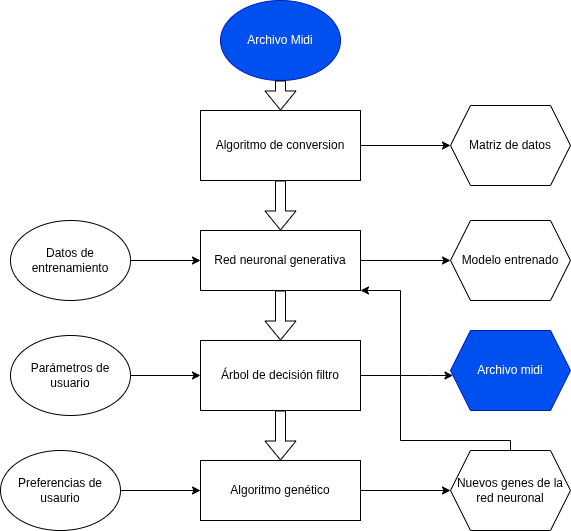
\includegraphics[width=0.5\textwidth]{img/arquitecturaia.png} 
    \end{center}
    \caption{Arquitectura de la aplicación}
    \label{fig:teclado_do_mayor} % Añadir una etiqueta para referencias cruzadas
\end{figure}




\section{Formalización de la Representación Matricial Relativa}

La piedra angular de la presente investigación reside en la transición de un modelo de datos basado en eventos absolutos —típico de los sistemas de Inteligencia Artificial que operan sobre el estándar MIDI tradicional— hacia un paradigma de representación matricial relativa. Esta formalización no busca meramente codificar la altura de las notas, sino capturar la semántica subyacente de la armonía funcional y la jerarquía tonal. 

Como se observa en el desarrollo del módulo \texttt{procesador\_midi.py}, la música no se trata como una sucesión estadística de números de nota (0-127), sino como un sistema de relaciones vectoriales. La importancia de este enfoque radica en la \textit{invarianza tonal}: la capacidad de un modelo de aprendizaje profundo para reconocer una progresión armónica o una línea melódica independientemente de la tónica en la que se ejecute. Según \cite{tymoczko2011}, la música occidental se organiza en espacios geométricos donde la proximidad no es solo acústica, sino funcional; nuestra representación matricial formaliza esta proximidad mediante el cálculo dinámico de grados y distancias interválicas.

\subsection{Abstracción de datos: Del evento absoluto al vector relativo}

El proceso de abstracción comienza con la deconstrucción del archivo MIDI. Mientras que el estándar MIDI define una nota mediante un entero absoluto $p \in [0, 127]$, nuestro sistema descompone esta variable en dos componentes críticos: la \textbf{Clase de Altura} (\textit{Pitch Class}) y el \textbf{Grado Escalar}.

En el código fuente de \texttt{procesador\_midi.py}, esta abstracción se materializa en la extracción inicial de la clase de altura mediante la operación de módulo:

\begin{verbatim}
# Extracción de la clase de altura en procesador_midi.py
midi_pitch = note['pitch']
pitch_class = midi_pitch % 12
row.append(float(pitch_class))
\end{verbatim}

Sin embargo, el \texttt{pitch\_class} por sí solo es insuficiente para la composición profesional. La abstracción propuesta añade una dimensión de temporalidad relativa. En lugar de utilizar marcas de tiempo absolutas (ticks), el sistema normaliza la duración basándose en la resolución del archivo (\texttt{ticks\_per\_beat}), permitiendo que el modelo aprenda ritmos independientemente del \textit{tempo} (BPM) seleccionado:

\begin{verbatim}
# Normalización rítmica relativa
duration_units = note['duration'] / ticks_per_unit
row.append(round(duration_units, 2))
\end{verbatim}

Esta primera capa de abstracción transforma un evento discreto en un vector bi-dimensional inicial $[PC, D]$, donde $PC$ es la clase de altura y $D$ es la duración relativa. Este paso es fundamental para mitigar el problema de la dispersión de datos en redes neuronales; al reducir el dominio de 128 notas a 12 clases de altura normalizadas rítmicamente, se facilita la convergencia del entrenamiento \cite{briot2020deep}.

\subsection{Algoritmo de mapeo de funciones armónicas y distancias interválicas}

El núcleo innovador del conversor es el algoritmo de mapeo de grados escalares. A diferencia de modelos como \textit{MusicTransformer} \cite{huang2018music}, que dependen de la atención posicional para inferir la tonalidad, nuestro sistema inyecta el conocimiento teórico de la escala directamente en la matriz de entrada.

La función \texttt{get\_scale\_degree} implementa un mapeo matemático que proyecta la nota actual sobre el espacio de la tónica definida. Sea $P$ la clase de altura de la nota, $T$ la tónica y $S$ el conjunto de intervalos de la escala (ej. $S_{Mayor} = \{0, 2, 4, 5, 7, 9, 11\}$). El Grado Escalar $G$ se define como:

\begin{equation}
R = (P - T) \mod 12
\end{equation}
\begin{equation}
G = 
\begin{cases} 
index(R, S) + 1 & \text{si } R \in S \\
(i + 1) + 0.5 & \text{si } S_i < R < S_{i+1} \\
|S| + 0.5 & \text{si } R > max(S)
\end{cases}
\end{equation}

Esta lógica permite manejar no solo notas diatónicas (grados enteros), sino también notas cromáticas o "alteraciones accidentales" (grados fraccionarios), lo cual es esencial para el contrapunto avanzado y la armonía de intercambio modal. El código implementa esta jerarquía de la siguiente manera:

\begin{verbatim}
def get_scale_degree(pitch_class, root_note, scale_intervals):
    relative_pitch = (pitch_class - root_note) % 12
    
    if relative_pitch in scale_intervals:
        return float(scale_intervals.index(relative_pitch) + 1)
    
    for i in range(len(scale_intervals) - 1):
        lower = scale_intervals[i]
        upper = scale_intervals[i+1]
        if lower < relative_pitch < upper:
            return float((i + 1) + 0.5)
    # ... (manejo de bordes)
\end{verbatim}

Adicionalmente, se integra el cálculo de la \textbf{distancia interválica relativa} entre notas consecutivas. Esta columna de la matriz permite que el algoritmo genético evalúe la "suavidad" de la conducción de voces (\textit{voice leading}). En \texttt{procesador\_midi.py}, el intervalo se normaliza a unidades de tono (donde 0.5 es un semitono), alineándose con la teoría de \cite{chew2014mathematical} sobre el modelado matemático de la tensión melódica:

\begin{verbatim}
# Cálculo de intervalo relativo en tonos
semitones = midi_pitch - last_note_pitch
interval = semitones / 2.0
row.append(interval)
\end{verbatim}

\subsection{Normalización y preparación del dataset para el entrenamiento}

La fase final de la formalización es la estructuración de la matriz resultante para su consumo por arquitecturas de aprendizaje profundo (RNN/LSTM). La matriz final posee una topología de $N \times 4$, donde cada fila representa un evento musical con cuatro parámetros:
\begin{enumerate}
    \item \textbf{Clase de Altura (Absoluta Octava):} Proporciona el color de la nota dentro del total cromático.
    \item \textbf{Duración (Relativa):} Cuantiza el ritmo en unidades de tiempo musical (corcheas, semicorcheas).
    \item \textbf{Grado Escalar (Funcional):} Define la posición de la nota respecto a la jerarquía de la escala, facilitando el aprendizaje de resoluciones armónicas.
    \item \textbf{Intervalo (Melódico):} Captura el movimiento horizontal de la voz.
\end{enumerate}

La preparación del dataset implica la vectorización de estas matrices. Dado que las redes recurrentes requieren secuencias de longitud fija, se implementa un sistema de \textit{sliding window} (ventana deslizante). Sin embargo, a diferencia de otros datasets simbólicos que solo guardan la nota, nuestra preparación conserva la \textbf{metadata de la tonalidad}. 

Esto permite realizar una \textit{normalización tonal activa}: durante el entrenamiento, se pueden trasponer todas las piezas a una tónica común de forma matemática, garantizando que el modelo aprenda que un grado "5.0" (Dominante) siempre tiende a resolver a un "1.0" (Tónica), independientemente de si la pieza original estaba en Fa sostenido o Do mayor. Este proceso es fundamental para alcanzar el objetivo de "generación paramétrica estructuralmente coherente" planteado en el Capítulo 1, ya que reduce drásticamente el espacio de búsqueda del algoritmo genético al operar sobre un dataset pre-estructurado bajo leyes armónicas \cite{hadjeres2017deepbach}.

\begin{verbatim}
# Estructura final de la fila de la matriz para entrenamiento
# [PitchClass, DurationUnits, ScaleDegree, IntervalTones]\end{algorithmic}
result_matrix = midi_to_matrix(target_file, root_note_name='C', scale_type='major')
\end{verbatim}

En conclusión, el conversor implementado no es solo una herramienta de transformación de formato, sino un motor de extracción de características teóricas. La representación resultante permite que el sistema híbrido de IA actúe como un compositor instruido que "entiende" la función de cada nota dentro de un contexto tonal, superando las limitaciones de la generación estocástica convencional.

\section{Diseño del Núcleo Generativo}
El núcleo generativo del sistema propuesto se fundamenta en una arquitectura híbrida que combina el aprendizaje profundo con mecanismos de control determinista. El componente central de esta arquitectura es una red neuronal recurrente diseñada para procesar y predecir secuencias de eventos musicales representados mediante una estructura matricial relativa. Este enfoque permite que el sistema no solo aprenda patrones melódicos estadísticos, sino que también mantenga una coherencia teórica al operar sobre intervalos y grados de la escala en lugar de valores absolutos.

\subsection{Estructura e Implementación de la Red Neuronal Generativa}

El núcleo generativo del sistema de composición automatizada se fundamenta en una red neuronal artificial híbrida construida y compilada de manera paramétrica mediante la función \texttt{build\_dynamic\_model} en el módulo \texttt{constructor\_red.py}. La entrada del modelo está diseñada para consumir tensores secuenciales de dimensiones $(L, F)$, donde $L$ (SEQ\_LENGTH) representa la longitud de la ventana temporal (fijada en 4 notas o eventos musicales previos) y $F$ (NUM\_FEATURES) representa la dimensión del vector de características por nota (fijada en 4 parámetros: clase de altura, duración rítmica, grado de la escala diatónica activa e intervalo en tonos respecto a la nota previa).

La arquitectura profunda está organizada en una topología secuencial secuenciada a través de las siguientes capas especializadas:
\begin{enumerate}
    \item \textbf{Capa de Convolución Temporal (Conv1D):} Recibe el tensor de entrada y actúa como un extractor de características locales a nivel de sub-frase musical. Utiliza 32 filtros y un tamaño de kernel de 2. Esta capa extrae patrones intervalares y de contorno rítmico inmediatos antes de alimentar las unidades recurrentes.
    \item \textbf{Capa de Memoria a Corto y Largo Plazo (LSTM):} Compuesta por 64 unidades con función de activación ReLU. Esta capa recurrente captura las dependencias temporales y la memoria formal a largo plazo de la secuencia musical, permitiendo mantener la coherencia armónica a lo largo de los compases. Si se definen múltiples capas recurrentes en la matriz, el sistema infiere y activa de forma automática el parámetro \texttt{return\_sequences=True} en las capas previas.
    \item \textbf{Capa de Regularización (Dropout):} Aplica una tasa de descarte aleatorio de conexiones de $0.20$ ($20\%$). Esta capa actúa como un regulador indispensable para evitar el sobreajuste (overfitting) del modelo ante la memorización directa del conjunto de entrenamiento.
    \item \textbf{Capa Densa Intermedia (Dense):} Una capa totalmente conectada compuesta por 32 neuronas con activación ReLU, la cual actúa como un extractor de representaciones abstractas finales antes de la síntesis de salida.
    \item \textbf{Capa de Salida (Dense con Regresión):} A diferencia de los modelos clasificadores de lenguaje tradicionales, esta capa final consta de un número de unidades igual a \texttt{NUM\_FEATURES} (4 neuronas) con una función de activación lineal. Esto convierte el problema en una regresión lineal multivariada, estimando valores continuos para los cuatro atributos de la siguiente nota.
\end{enumerate}

El modelo se compila utilizando el optimizador Adam, el cual aplica tasas de aprendizaje adaptativas para acelerar la convergencia, y la función de pérdida del error cuadrático medio (MSE), alineada con la naturaleza continua del espacio métrico y de alturas. Este diseño permite que la red proponga melodías fluidas e inéditas basadas en la herencia estilística de los datos de entrada, las cuales son posteriormente normalizadas y corregidas por la capa del árbol de decisión determinista.

\subsection{Arquitectura de la red neuronal}
La arquitectura implementada utiliza un modelo de tipo \textit{Sequential} basado en redes de Memoria a Corto y Largo Plazo (LSTM), seleccionadas por su capacidad superior para capturar dependencias temporales en secuencias musicales. La estructura de la red se define de la siguiente manera:

\begin{enumerate}
    \item \textbf{Capa de Entrada:} Recibe tensores con una forma de $(L, F)$, donde $L$ (SEQ\_LENGTH) es la longitud de la secuencia (fijada en 4 eventos) y $F$ (NUM\_FEATURES) es el número de características por evento.
    \item \textbf{Capa LSTM:} Una capa de 64 unidades con función de activación ReLU. Esta capa procesa la secuencia temporal y retorna un vector de características que resume el contexto musical previo.
    \item \textbf{Capa Densa Intermedia:} Una capa totalmente conectada de 32 neuronas con activación ReLU, que actúa como un extractor de características de alto nivel para refinar la predicción.
\end{enumerate}

El modelo utiliza el optimizador \textit{Adam} y una función de pérdida de error cuadrático medio (MSE), lo que orienta el aprendizaje hacia un problema de regresión para la estimación precisa de los parámetros musicales.

\subsection{Capas paramétricas enlazadas a genes}
En el contexto de la arquitectura híbrida, las características de entrada y salida de la red actúan como los "genes" que definen la identidad del material musical generado. El sistema utiliza una representación de 4 características fundamentales (genes paramétricos):
\begin{itemize}
    \item \textbf{Nota:} Valor de altura relativo.
    \item \textbf{Duración:} Magnitud temporal del evento.
    \item \textbf{Grado:} Posición dentro de la escala diatónica activa.
    \item \textbf{Intervalo:} Distancia semitonal respecto a la nota anterior.
\end{itemize}
Estos parámetros permiten que el algoritmo genético, mencionado en el planteamiento del problema, opere directamente sobre la configuración de la red, ajustando las tendencias generativas según las preferencias estéticas del usuario y las restricciones de los árboles de decisión.

\subsection{Definición de la capa de salida}
La capa de salida consiste en una capa densa con un número de unidades igual a \texttt{NUM\_FEATURES} (4). A diferencia de los modelos de clasificación categórica comunes en la generación de texto, esta capa utiliza una activación lineal para realizar una \textbf{regresión multivariada}. Los cuatro valores continuos resultantes representan la predicción del próximo evento en el espacio paramétrico definido. Este diseño permite una mayor fluidez en la generación de duraciones e intervalos, los cuales son posteriormente post-procesados y cuantizados por el sistema de reglas para asegurar su validez dentro de la teoría musical convencional.

\section{Implementación de Filtros Deterministas}

En los sistemas contemporáneos de composición automatizada e inteligencia artificial aplicada a la música, uno de los desafíos teóricos y prácticos más significativos radica en la conciliación del comportamiento estocástico y creativo de los modelos de aprendizaje profundo con las restricciones normativas y formales descritas por la teoría musical clásica. Las redes neuronales profundas, tales como las redes de memoria a corto y largo plazo (LSTM) o los modelos basados en mecanismos de atención (Transformers), demuestran una capacidad sobresaliente para aprender representaciones complejas, transiciones de probabilidad y estilos a partir de corpus masivos de datos. Sin embargo, al estar fundamentadas en optimizaciones probabilísticas y de mínimos cuadrados (tales como la pérdida del error cuadrático medio, MSE), estas redes carecen intrínsecamente de un mecanismo determinista para garantizar el cumplimiento de restricciones rígidas (`hard constraints`). 

Por ejemplo, una red neuronal entrenada para la generación melódica puede sugerir un intervalo de novena menor o una nota extremadamente disonante fuera de la escala base simplemente porque la distribución de probabilidad local del modelo de lenguaje musical presentaba un residuo estocástico propicio en dicho punto. Si bien este comportamiento puede ser tolerado en contextos de improvisación libre o música contemporánea no tonal, resulta inaceptable bajo los marcos de la armonía tonal académica y el contrapunto estricto, donde errores como la resolución incorrecta de disonancias o la existencia de saltos melódicos no cantables invalidan la estructura de la pieza.

Para resolver esta limitación, el presente trabajo introduce una arquitectura híbrida de carácter neurosimbólico, estructurada en múltiples capas. En esta arquitectura, el componente de aprendizaje profundo (la red neuronal generativa parametrizada) actúa como un motor creativo de exploración libre que propone secuencias de notas candidatas con base en el estilo aprendido del conjunto de datos. Simultáneamente, el componente simbólico, constituido por un filtro determinista estructurado como un árbol de decisión parametrizable, interviene en la salida del modelo generativo. Este árbol actúa como un validador normativo de tipo "`hard constraint satisfaction`" (satisfacción de restricciones duras) que evalúa y modifica localmente la secuencia musical antes de su codificación en formato MIDI.

El ciclo dinámico de inferencia y post-procesamiento híbrido se formaliza de la siguiente manera. Sea una melodía candidata generada por la red neuronal expresada como una matriz $\mathbf{M} \in \mathbb{R}^{N \times 4}$, donde cada fila $j \in \{0, 1, \dots, N-1\}$ representa un evento musical compuesto por el vector:
\begin{equation}
    \mathbf{v}_j = [pc_j, d_j, deg_j, int_j]
\end{equation}
Donde $pc_j$ es la clase de altura (pitch class), $d_j$ es la duración temporal en unidades relativas de semicorchea, $deg_j$ representa el grado relativo a la escala activa, y $int_j$ es el intervalo en tonos respecto a la nota inmediatamente anterior. La matriz pasa a través de la función de filtrado determinista del árbol de decisión $f_{\text{árbol}}: \mathbb{R}^{N \times 4} \to \mathbb{R}^{N \times 4}$, la cual evalúa y corrige las desviaciones respecto a los límites teóricos parametrizados por el usuario. 

A diferencia de los enfoques tradicionales de generación restringida, los cuales descartan por completo las secuencias que no cumplen con los requisitos mínimos (lo que genera un costo computacional inasumible debido a la continua re-generación estocástica), el árbol de decisión propuesto opera bajo una estrategia de "reparación local". El árbol identifica el punto exacto de la desviación normativa y aplica una corrección matemática directa sobre la nota conflictiva y sus vecindades. Esto preserva la coherencia temática del modelo neuronal mientras asegura el cumplimiento inequívoco de las leyes de la teoría armónica.

\subsection{Codificación de tonalidades, modos e inducción de mutaciones}

Para parametrizar matemáticamente el comportamiento del filtro y del algoritmo genético, se requiere una formalización algebraica estricta del espacio de alturas y modos musicales. La clase de alturas (pitch class) se modela sobre el anillo cociente $\mathbb{Z}_{12} = \{0, 1, 2, \dots, 11\}$, donde cada entero representa una nota musical del temperamento igual, tomando a Do ($C$) como el origen de coordenadas $0$:
\begin{equation}
    C \equiv 0, \quad C\# \equiv 1, \quad D \equiv 2, \quad \dots, \quad B \equiv 11
\end{equation}

La tónica de la escala se codifica mediante un parámetro entero $T \in \{1, 2, \dots, 12\}$, el cual se transforma linealmente al espacio $\mathbb{Z}_{12}$ a través de la función de proyección:
\begin{equation}
    t_0 = (T - 1) \pmod{12}
\end{equation}
Esta tónica sirve como el origen tonal absoluto de la composición.

Los modos eclesiásticos o modos griegos diatónicos se codifican mediante un parámetro de modo $M \in \{1, 2, \dots, 7\}$. Cada modo $M$ se define matemáticamente como un conjunto ordenado de siete intervalos relativos $\mathcal{I}_M = \{i_0, i_1, \dots, i_6\} \subset \mathbb{Z}_{12}$ que representan las distancias en semitonos desde el centro tonal $t_0$. Los modos se estructuran algebraicamente según los siguientes vectores de intervalos:
\begin{align}
    \mathcal{I}_1 \text{ (Jónico)} &= \{0, 2, 4, 5, 7, 9, 11\} \\
    \mathcal{I}_2 \text{ (Dórico)} &= \{0, 2, 3, 5, 7, 9, 10\} \\
    \mathcal{I}_3 \text{ (Frigio)} &= \{0, 1, 3, 5, 7, 8, 10\} \\
    \mathcal{I}_4 \text{ (Lidio)} &= \{0, 2, 4, 6, 7, 9, 11\} \\
    \mathcal{I}_5 \text{ (Mixolidio)} &= \{0, 2, 4, 5, 7, 9, 10\} \\
    \mathcal{I}_6 \text{ (Eólico)} &= \{0, 2, 3, 5, 7, 8, 10\} \\
    \mathcal{I}_7 \text{ (Locrio)} &= \{0, 1, 3, 5, 6, 8, 10\}
\end{align}

Dado un par de parámetros $(T, M)$, la escala diatónica activa en el sistema se denota como el conjunto $\mathcal{D}_{T,M} \subset \mathbb{Z}_{12}$, definido formalmente como la traslación del conjunto de intervalos modales respecto a la tónica:
\begin{equation}
    \mathcal{D}_{T,M} = \{ (t_0 + i) \pmod{12} \mid i \in \mathcal{I}_M \}
\end{equation}

Una nota representada por una clase de altura $pc$ se define como diatónica si y solo si $pc \in \mathcal{D}_{T,M}$. En caso contrario, se define como una nota cromática o no diatónica.

En el marco evolutivo del sistema, el algoritmo genético interactivo opera sobre una población de cromosomas. Cada cromosoma es una matriz de melodía $\mathbf{M}$ de dimensiones $N \times 4$. La optimización de la red neuronal y la búsqueda de trayectorias melódicas estéticas dependen de los operadores genéticos de cruce y mutación aplicados a estas matrices. 

El operador de cruce (crossover) recibe dos matrices progenitoras $\mathbf{P}_A, \mathbf{P}_B \in \mathbb{R}^{N \times 4}$ y genera un hijo $\mathbf{H} \in \mathbb{R}^{N \times 4}$ mediante un corte de punto único. Sea $k \in \{1, 2, \dots, N-2\}$ un punto de corte aleatorio. El hijo resultante se construye mediante la concatenación vertical:
\begin{equation}
    \mathbf{H} = \begin{bmatrix} \mathbf{P}_A[0 \dots k-1] \\ \mathbf{P}_B[k \dots N-1] \end{bmatrix}
\end{equation}

El operador de mutación introduce variabilidad en el cromosoma con una probabilidad por gen de $p_m$. Para asegurar que las mutaciones generen individuos que posean sentido biológico y técnico para la red neuronal recurrente, las mutaciones se especializan de acuerdo a las características físicas del parámetro alterado:
\begin{enumerate}
    \item \textbf{Mutación de la Duración ($d_j$):} Si el parámetro rítmico de la nota en la posición $j$ es seleccionado para mutar, su valor se altera aleatoriamente sustituyéndose por un elemento del conjunto discreto de duraciones musicales válidas:
    \begin{equation}
        d_j \in \mathcal{U}_{\text{duraciones}} = \{0.25, 0.50, 0.75, 1.00, 1.50, 2.00, 3.00, 4.00\}
    \end{equation}
    Este conjunto discreto representa subdivisiones que van desde la semicorchea ($0.25$) hasta la redonda ($4.00$) en términos relativos, asegurando la consistencia rítmica de la partitura.
    
    \item \textbf{Mutación de la Altura ($pc_j$) con sentido estructural:} Si la altura de la nota en la posición $j$ muta, el sistema selecciona de manera uniforme un nuevo valor de clase de altura $pc'_j \in \mathcal{D}_{T,M}$. La asignación directa de una nota arbitraria destruiría la coherencia interválica local de la melodía y generaría saltos melódicos no deseados de gran amplitud. Para evitar este efecto, se calcula la diferencia en semitonos $\delta \in \mathbb{Z}$ entre la nueva nota y la nota antigua:
    \begin{equation}
        \delta = pc'_j - pc_j
    \end{equation}
    Esta diferencia se normaliza al intervalo diatónico más corto mediante:
    \begin{equation}
        \delta_n = \begin{cases} \delta - 12 & \text{si } \delta > 6 \\ \delta + 12 & \text{si } \delta \le -6 \\ \delta & \text{en otro caso} \end{cases}
    \end{equation}
    
    Para inducir la mutación de forma que "haga sentido" al codificador y al decodificador matricial, el algoritmo actualiza localmente tres variables de la matriz de forma simultánea:
    \begin{itemize}
        \item La clase de altura del gen mutado se actualiza: $pc_j \leftarrow pc'_j$.
        \item El grado de la escala se re-calcula usando la función de correspondencia diatónica: $deg_j \leftarrow g(pc'_j, t_0, \mathcal{I}_M)$.
        \item Se ajustan de forma balanceada las relaciones interválicas adyacentes para encapsular la mutación. El intervalo en tonos del evento actual se incrementa sumando la mitad de la desviación de semitonos:
        \begin{equation}
            int_j \leftarrow int_j + \frac{\delta_n}{2}
        \end{equation}
        Para evitar que esta alteración desplace de forma absoluta e indeseada todas las notas subsiguientes de la melodía (lo que arruinaría la progresión temática previa), se sustrae exactamente la misma cantidad al intervalo de la siguiente nota:
        \begin{equation}
            int_{j+1} \leftarrow int_{j+1} - \frac{\delta_n}{2}
        \end{equation}
        Si $j = N-1$ (la última nota de la secuencia), solo se altera $int_j$. Este mecanismo de conservación garantiza la preservación del contorno de alturas absoluto aguas abajo de la mutación.
    \end{itemize}
\end{enumerate}

\subsection{Lógica de poda y validación de secuencias candidatas}

El proceso de validación y poda de las melodías candidatas propuestas por el modelo estocástico se efectúa de manera secuencial a través de un árbol de decisión determinista. Este árbol analiza cada evento melódico y sus relaciones interválicas previas para detectar violaciones a las restricciones tonales y de conducción de voces.

En la teoría de conducción de voces y contrapunto, los intervalos musicales se clasifican rigurosamente por su amplitud física en semitonos absolutos $\Delta = |p_t - p_{t-1}|$:
\begin{itemize}
    \item \textbf{Paso o Grado Conjunto (Step):} Movimiento de $1$ o $2$ semitonos (segunda menor o segunda mayor). Representa la máxima suavidad melódica.
    \item \textbf{Salto Corto (Skip):} Movimiento de $3$ o $4$ semitonos (tercera menor o tercera mayor). Introduce una tensión moderada pero fluida.
    \item \textbf{Salto Largo (Leap):} Movimiento de $5$ o más semitonos (cuarta justa, quinta justa o mayores). Introduce una gran tensión y debe resolverse de forma contraria para mantener la cantabilidad.
\end{itemize}

El árbol de decisión opera sobre la secuencia melódica aplicando un algoritmo recursivo de validación. La lógica interna de este árbol se describe mediante la secuencia de pruebas lógicas y ramificaciones condicionales estructuradas a continuación:

\begin{verbatim}
\caption{Algoritmo del Árbol de Decisión para Corrección de Melodías}
\begin{algorithmic}[1]
\REQUIRE Matriz de melodía original $\mathbf{M}$, parámetros $T, M, \text{max\_skips}, \text{max\_leaps}, \text{max\_non\_diatonic}$
\ENSURE Matriz de melodía filtrada y corregida $\mathbf{M}'$
\STATE Obtener la escala diatónica activa $\mathcal{D}_{T,M}$ y la tónica $t_0$.
\STATE Inicializar contadores: $c_{\text{crom}} \leftarrow 0$, $c_{\text{skips}} \leftarrow 0$, $c_{\text{leaps}} \leftarrow 0$.
\STATE Reconstruir las alturas MIDI absolutas $P = \{p_0, p_1, \dots, p_{N-1}\}$ a partir de la columna de intervalos de $\mathbf{M}$.
\FOR{$i = 0$ \TO $N-1$}
    \STATE $pc \leftarrow p_i \pmod{12}$
    \COMMENT{\textbf{Nodo de Decisión 1: Diatonicidad}}
    \IF{$pc \notin \mathcal{D}_{T,M}$}
        \COMMENT{\textbf{Nodo de Decisión 2: Límite Cromático}}
        \IF{$c_{\text{crom}} \ge \text{max\_non\_diatonic}$}
            \STATE Modificar $p_i \leftarrow \text{get\_nearest\_diatonic}(p_i, \mathcal{D}_{T,M})$
            \STATE Actualizar $pc \leftarrow p_i \pmod{12}$
        \ELSE
            \STATE $c_{\text{crom}} \leftarrow c_{\text{crom}} + 1$
        \ENDIF
    \ENDIF
    \IF{$i > 0$}
        \STATE $\text{intervalo} \leftarrow p_i - p_{i-1}$
        \STATE $\Delta \leftarrow |\text{intervalo}|$
        \COMMENT{\textbf{Nodo de Decisión 3: Clasificación de Saltos}}
        \IF{$\Delta \in \{3, 4\}$}
            \COMMENT{\textbf{Nodo de Decisión 4: Límite de Skips}}
            \IF{$c_{\text{skips}} \ge \text{max\_skips}$}
                \STATE $\text{dirección} \leftarrow \text{signo}(\text{intervalo})$
                \STATE $\text{step\_size} \leftarrow \text{diatonic\_step}(p_{i-1}, \text{dirección}, \mathcal{D}_{T,M})$
                \STATE $p_i \leftarrow p_{i-1} + \text{dirección} \times \text{step\_size}$
                \STATE Asegurar $p_i$ diatónico.
            \ELSE
                \STATE $c_{\text{skips}} \leftarrow c_{\text{skips}} + 1$
            \ENDIF
        \ELSIF{$\Delta \ge 5$}
            \COMMENT{\textbf{Nodo de Decisión 5: Límite de Leaps}}
            \IF{$c_{\text{leaps}} \ge \text{max\_leaps}$}
                \STATE $\text{dirección} \leftarrow \text{signo}(\text{intervalo})$
                \COMMENT{\textbf{Intento de degradación suave a Skip}}
                \IF{$c_{\text{skips}} < \text{max\_skips}$}
                    \STATE $p_i \leftarrow p_{i-1} + \text{dirección} \times 3$
                    \IF{$p_i \pmod{12} \notin \mathcal{D}_{T,M}$}
                        \STATE $p_i \leftarrow p_{i-1} + \text{dirección} \times 4$
                    \ENDIF
                    \STATE Asegurar $p_i$ diatónico.
                    \STATE $c_{\text{skips}} \leftarrow c_{\text{skips}} + 1$
                \ELSE
                    \COMMENT{\textbf{Forzar reducción estricta a Step}}
                    \STATE $\text{step\_size} \leftarrow \text{diatonic\_step}(p_{i-1}, \text{dirección}, \mathcal{D}_{T,M})$
                    \STATE $p_i \leftarrow p_{i-1} + \text{dirección} \times \text{step\_size}$
                    \STATE Asegurar $p_i$ diatónico.
                \ENDIF
            \ELSE
                \STATE $c_{\text{leaps}} \leftarrow c_{\text{leaps}} + 1$
            \ENDIF
        \ENDIF
    \ENDIF
\ENDFOR
\STATE Re-calcular los parámetros de la matriz $\mathbf{M}'$ basándose en las nuevas alturas corregidas $P$.
\RETURN $\mathbf{M}'$
\end{verbatim}

La función $\text{diatonic\_step}(pitch, dir, \text{escala})$ calcula la distancia al siguiente grado de la escala en la dirección indicada. Si la escala activa requiere un movimiento de $2$ semitonos, la función retorna $2$. Si el grado diatónico se encuentra a una distancia de segunda menor, retorna $1$.

Este mecanismo de poda asegura que si la red neuronal propone una melodía que salta abruptamente de forma repetida (ej. una sucesión de quintas y octavas disjuntas), el árbol de decisión interviene y "poda" la curva melódica, aproximando las notas a pasos diatónicos más cercanos. La validación se realiza de forma secuencial y cronológica para imitar el proceso humano de corrección y revisión melódica.

\subsection{Interfaz de parametrización: Tonalidad y modo}

El control creativo del sistema híbrido se canaliza mediante una interfaz de parametrización interactiva que actúa sobre los umbrales lógicos del árbol de decisión y los operadores evolutivos. Esta parametrización otorga al usuario un control exhaustivo sobre el nivel de disonancia, la agilidad de los saltos y el rigor estructural del material generado. 

La parametrización se gestiona de forma interactiva y permite regular las siguientes restricciones fundamentales:
\begin{table}[H]
\centering
\caption{Parámetros de la interfaz condicional del filtro armónico.}
\label{tab:harmonic-filter-parameters}

\begin{tabular}{|l|c|p{8cm}|}
\hline
\textbf{Parámetro} &
\textbf{Rango de Entrada} &
\textbf{Efecto en la Salida Melódica}
\\ \hline

\texttt{tonic} &
$1 \leq T \leq 12$ &
Define el centro tonal absoluto de la composición.
\\ \hline

\texttt{greek\_mode} &
$1 \leq M \leq 7$ &
Selecciona la distribución intervalar diatónica correspondiente al modo griego.
\\ \hline

\texttt{max\_skips} &
$\geq 0$ &
Controla la cantidad máxima de intervalos de tercera (3 o 4 semitonos).
\\ \hline

\texttt{max\_leaps} &
$\geq 0$ &
Controla la cantidad máxima de saltos amplios ($\geq 5$ semitonos).
\\ \hline

\texttt{max\_non\_diatonic} &
$\geq 0$ &
Regula la presencia de notas cromáticas o alteraciones accidentales.
\\ \hline

\end{tabular}
\end{table}


La interacción de estos parámetros define el comportamiento del sistema en un continuo que va desde la rigidez académica hasta la experimentación libre:
\begin{itemize}
    \item \textbf{Configuración de Contrapunto Estricto:} Si el usuario parametriza $\text{max\_non\_diatonic} = 0$, $\text{max\_leaps} = 0$ y $\text{max\_skips} = 2$, el árbol de decisión podará de forma agresiva cualquier intento del modelo neuronal de realizar cromatismos o saltos melódicos pronunciados. El resultado será una melodía suave, principalmente por grados conjuntos, muy alineada con el estilo vocal del Renacimiento y las reglas de conducción clásicas.
    
    \item \textbf{Configuración de Expresividad Cromática Moderada:} Al relajar los parámetros a $\text{max\_non\_diatonic} = 3$, $\text{max\_skips} = 5$ y $\text{max\_leaps} = 2$, el árbol de decisión amplía su umbral de tolerancia. Esto permite la aparición controlada de notas accidentales de paso y saltos expresivos (ej. intervalos de quinta o sexta justa), dotando a la melodía de una estética más cercana al romanticismo o al jazz modal, sin llegar a colapsar en la atonalidad desorganizada.
\end{itemize}

Esta modularidad demuestra que la arquitectura neurosimbólica no limita la expresividad artística de la red neuronal. Por el contrario, la encauza mediante un conjunto dinámico de directrices técnicas controladas por el compositor. Esto permite al investigador explorar diferentes estilos musicales y regular de manera precisa el equilibrio entre la exploración probabilística del modelo recurrente y la explotación normativa del sistema de reglas simbólicas.

\section{Optimización Evolutiva}

La generación de material musical mediante inteligencia artificial a menudo se enfrenta al problema de la formalización objetiva de la estética. Mientras que la precisión técnica de una red neuronal puede medirse mediante pérdidas matemáticas tradicionales, las cualidades expresivas y estilísticas del arte son esquivas a las métricas computacionales puras. Para solventar este distanciamiento entre la cuantificación algorítmica y la valoración artística, se integra un Algoritmo Genético Interactivo (IGA, por sus siglas en inglés). Esta técnica evolutiva incorpora al compositor directamente en el bucle de optimización ("`human-in-the-loop`"), utilizando la preferencia humana como la función de aptitud o \textit{fitness} que guía el proceso selectivo y dirige la convergencia de la población hacia territorios melódicos estéticamente satisfactorios.

El ciclo evolutivo del algoritmo propuesto sigue un flujo estructurado de cinco etapas:
\begin{enumerate}
    \item \textbf{Inicialización:} Se genera una población inicial de 10 cromosomas (matrices de melodía) de forma aleatoria, bajo las restricciones diatónicas básicas de la tonalidad y modo seleccionados.
    \item \textbf{Evaluación y Selección Interactiva:} El usuario analiza las melodías representadas simbólicamente y selecciona de forma directa aquellos individuos que se alinean con sus preferencias estéticas.
    \text{Backup de Generación:} Las matrices seleccionadas y el resto de la población se guardan en un registro histórico indexado temporalmente para permitir auditorías y retrocesos.
    \item \textbf{Cruce (Crossover):} Se eligen aleatoriamente parejas de padres del grupo seleccionado y se recombinan para heredar estructuras motivacionales a los descendientes.
    \item \textbf{Mutación:} Se introducen perturbaciones estocásticas localizadas en los genes de altura y duración rítmica, asegurando la diversidad genotípica y evitando la convergencia prematura.
\end{enumerate}

\subsection{Definición del cromosoma}

En el contexto de este algoritmo, el genotipo de cada individuo melódico se codifica mediante un cromosoma matricial $\mathbf{M} \in \mathbb{R}^{N \times 4}$, donde $N$ representa la longitud de la melodía expresada en número de notas consecutivas. Cada locus $j \in \{0, 1, \dots, N-1\}$ dentro del cromosoma representa un gen compuesto por cuatro alelos específicos que determinan la física de la nota musical:
\begin{equation}
    \mathbf{g}_j = \big[ pc_j, d_j, deg_j, int_j \big]
\end{equation}

Los alelos que componen cada gen se definen teóricamente a continuación:
\begin{itemize}
    \item \textbf{Clase de Altura ($pc_j \in \mathbb{Z}_{12}$):} Primer alelo, codificado como un entero modular que representa la nota musical en el temperamento igual de doce tonos. Captura la identidad absoluta de la nota en la octava base (ej. $0$ para Do, $7$ para Sol).
    \item \textbf{Duración Rítmica ($d_j \in \mathbb{R}^+$):} Segundo alelo, codificado como un valor real que representa la magnitud temporal del evento musical en unidades relativas, tomando como unidad base ($1.00$) la duración de una semicorchea o un pulso de subdivisión del reloj.
    \item \textbf{Grado Escalar ($deg_j \in \mathbb{R}$):} Tercer alelo, que indica el valor armónico relativo de la nota dentro de la escala activa. Es un número que identifica si la nota es diatónica estricta (ej. $1.0, 2.0, \dots$) o si presenta alteraciones cromáticas intermedias (ej. $1.5, 2.5$).
    \item \textbf{Intervalo Relativo ($int_j \in \mathbb{R}$):} Cuarto alelo, que describe la diferencia de altura en tonos entre la nota actual y la nota precedente. Este gen es fundamental para capturar el perfil de alturas o contorno melódico de la secuencia musical.
\end{itemize}

Esta estructura matricial híbrida destaca por su capacidad de representar de forma simultánea tanto las propiedades absolutas del evento musical ($pc_j, d_j$) como sus relaciones estructurales y gramaticales respecto al entorno y el tiempo ($deg_j, int_j$). Esto dota al cromosoma de una gran robustez frente a las operaciones de cruce y mutación, manteniendo la coherencia interna de los datos.

\subsection{Operadores genéticos: Cruce y mutación aplicados a la notación simbólica}

Los operadores de cruce y mutación son los encargados de guiar la exploración en el espacio de diseño melódico. En el sistema desarrollado, estos operadores se han adaptado de forma estricta a la notación simbólica y matricial del modelo.

El operador de cruce (crossover) hereda la estructura formal de las melodías progenitoras dividiendo las matrices en un punto de corte aleatorio. Dadas dos matrices progenitoras seleccionadas por el usuario, $\mathbf{P}_A$ y $\mathbf{P}_B$, el operador selecciona uniformemente un índice de nota $k \in \{1, 2, \dots, N-2\}$ y ensambla al hijo $\mathbf{H}$ según la ecuación:
\begin{equation}
    \mathbf{H} = \begin{bmatrix} \mathbf{P}_A[0 \dots k-1] \\ \mathbf{P}_B[k \dots N-1] \end{bmatrix}
\end{equation}
Este cruzamiento de bloque único permite preservar los pequeños motivos melódicos de $k$ notas provenientes del progenitor A, y la resolución temática o sección final proveniente del progenitor B, imitando de esta forma el desarrollo musical formal por frases.

El operador de mutación introduce variaciones estocásticas controladas en los alelos de altura y duración rítmica con una probabilidad de mutación de $p_m$. Para asegurar que la variación tenga sentido biológico y no genere atonalidad, el operador de mutación implementa las siguientes reglas específicas sobre los genes de la nota $j$:
\begin{itemize}
    \item \textbf{Mutación Rítmica:} Si se selecciona el alelo de duración $d_j$, se modifica su valor por otro miembro seleccionado al azar de la escala de subdivisiones convencionales:
    \begin{equation}
        d_j \leftarrow \text{random\_choice}(\{0.25, 0.50, 0.75, 1.00, 1.50, 2.00, 3.00, 4.00\})
    \end{equation}
    \item \textbf{Mutación de Altura Localizada:} Si el alelo de altura $pc_j$ es seleccionado, se escoge aleatoriamente una nueva clase de altura diatónica $pc'_j$ dentro de la escala activa $\mathcal{D}_{T,M}$. Para evitar que este cambio desplace de manera absoluta e indeseada todo el perfil de alturas de la melodía que le sigue, se ejecuta un ajuste interválico localizado. 
    
    Sea $\delta_n$ la distancia en semitonos normalizada más corta en la octava entre $pc'_j$ y $pc_j$. Se actualiza la clase de altura $pc_j \leftarrow pc'_j$ y se re-calcula su grado diatónico $deg_j$. Para absorber el salto localmente y que no se propague, se modifica el gen de intervalo del evento actual sumando el incremento de tonos:
    \begin{equation}
        int_j \leftarrow int_j + \frac{\delta_n}{2}
    \end{equation}
    Y se resta exactamente el mismo incremento al gen de intervalo de la nota siguiente:
    \begin{equation}
        int_{j+1} \leftarrow int_{j+1} - \frac{\delta_n}{2}
    \end{equation}
    Este par de correcciones contrapuestas cancela el desplazamiento acumulativo de tonos aguas abajo, manteniendo fija la afinación absoluta del resto de la melodía y encapsulando el efecto de la mutación a un único evento melódico.
\end{itemize}

\subsection{Interfaz de usuario para la selección de parámetros}

Para habilitar la interacción entre el compositor humano y el algoritmo genético, se desarrolla una interfaz interactiva de consola. Esta interfaz permite al usuario definir las bases físicas y armónicas del espacio de búsqueda antes de dar inicio al ciclo evolutivo de selección.

La interfaz de usuario implementa las siguientes funciones operativas principales:
\begin{enumerate}
    \item \textbf{Entrada de Parámetros de Escala:} Solicita al usuario definir la tónica tonal y la escala diatónica base. El usuario introduce valores enteros para la tónica ($1 \leq T \leq 12$, mapeados de Do a Si) y para el modo griego ($1 \leq M \leq 7$, mapeados de Jónico a Locrio). Esto configura la matriz de intervalos modales activos.

    \item \textbf{Visualización de Individuos en Tiempo Real:} Lee los archivos de texto correspondientes a los 10 individuos de la población y los convierte a una notación simbólica simplificada de notas y duraciones relativas (por ejemplo, $C(0.25)\rightarrow D(0.50)\rightarrow F(1.00)$). Esto permite al compositor leer y previsualizar rápidamente el contorno melódico y el ritmo de cada candidato.

    \item \textbf{Captura de Retroalimentación Estética:} Presenta una lista numerada del 1 al 10. El compositor introduce, mediante una entrada separada por comas, los índices de los individuos que desea seleccionar como padres de la siguiente generación (por ejemplo, \texttt{1,3,6}).

    \item \textbf{Gestión de Archivo Histórico:} Al ingresar la selección, la interfaz crea un subdirectorio con la fecha y hora actuales dentro de la carpeta \texttt{historial/} y copia las 10 matrices de la generación previa. Esta base de datos temporal asegura la trazabilidad del proceso creativo y permite analizar la deriva genética inducida por las decisiones artísticas del usuario.

    \item \textbf{Evolución y Escritura Automatizada:} Con base en los padres seleccionados, el sistema ejecuta los operadores de cruce y mutación localizada. Posteriormente, escribe los 10 nuevos individuos en archivos con formato \texttt{matrices\_entrada/individuo\_X.txt}, reemplazando los anteriores y preparando el entorno para la siguiente generación evolutiva.
\end{enumerate}

Este diseño interactivo desacopla la formulación matemática de los operadores evolutivos de la experiencia directa del usuario. Permite al músico interactuar directamente con la teoría contrapuntística y melódica de forma simbólica y creativa, guiando la deriva de las secuencias generadas hacia resultados estilísticamente valiosos y personalizados.

\section{Integración de la Arquitectura y Workflow}

La arquitectura del sistema propuesto se integra mediante un flujo de trabajo modular ("`workflow`"), estructurado en cuatro capas diferenciadas: la capa de adquisición e interpretación de datos, la capa generativa probabilística, la capa simbólica determinista y la capa evolutiva interactiva. Este diseño desacoplado permite aislar el procesamiento de señales físicas (archivos MIDI), la optimización matemática de redes profundas, la aplicación normativa de restricciones de armonía y la selección heurística basada en las preferencias estéticas del compositor. 

La integración formal del flujo de trabajo sigue una secuencia lineal y cíclica. En primer lugar, los datos del conjunto de entrenamiento son pre-procesados para su consumo por el modelo recurrente. Seguidamente, el compositor utiliza el algoritmo genético interactivo para guiar la deriva genotípica de las melodías candidatas. Las matrices seleccionadas por el compositor sirven de entrada y estímulo para la red neuronal recurrente, la cual propone nuevas secuencias de notas de forma autónoma. Finalmente, estas secuencias son tamizadas y corregidas en tiempo real por el filtro del árbol de decisión determinista, asegurando su coherencia antes de su exportación al pipeline de salida.

\subsection{Comunicación entre módulos}

La comunicación y transferencia de información entre los distintos componentes de la arquitectura se efectúa mediante una estructura de datos unificada: una matriz numérica bidimensional implementada como un arreglo de NumPy. Esta matriz posee una topología fija de $N \times 4$, donde cada fila representa un evento musical y las columnas corresponden a las variables relativas de nota, duración, grado de la escala e intervalo. Al utilizar la matriz como protocolo común de comunicación, se elimina la necesidad de serializaciones complejas o conversiones redundantes de formatos, garantizando la compatibilidad inmediata entre módulos escritos bajo distintos paradigmas.

El protocolo de transferencia de datos se describe según los siguientes flujos de comunicación entre archivos:
\begin{itemize}
    \item \textbf{De Señal Física a Matriz de Datos:} El módulo \texttt{procesador\_midi.py} analiza los archivos MIDI de entrada almacenados en el directorio \texttt{datos\_entrada/}, extrayendo los eventos de encendido (\textit{Note On}) y apagado (\textit{Note Off}). Convierte estos datos en matrices numéricas relativas compatibles con el optimizador y la red.
    \item \textbf{De Población Evolutiva a Datos de Entrenamiento:} El script \texttt{optimizador\_genetico.py} inicializa y evoluciona la población de cromosomas matriciales, guardando cada individuo de forma independiente en archivos de texto en la carpeta \texttt{matrices\_entrada/}.
    \item \textbf{De Matriz de Entrada a Red Neuronal:} El generador melódico \texttt{generador\_melodias.py} importa \texttt{constructor\_red.py} para construir la red recurrente a partir de la configuración matricial cargada desde \texttt{arquitectura\_tensor.txt}. Consume las matrices evolucionadas para entrenar el modelo y proponer nuevas predicciones.
    \item \textbf{De Predicción Estocástica a Validación Simbólica:} La matriz resultante de la red se transfiere directamente al módulo \texttt{filtro\_arbol\_decision.py}, donde es evaluada secuencialmente para corregir saltos melódicos o cromatismos no permitidos.
    \item \textbf{De Matriz Validada a Señal Física:} La matriz corregida por el árbol se transfiere de vuelta a \texttt{procesador\_midi.py} para su conversión final en archivos MIDI ejecutables.
\end{itemize}

\subsection{Pipeline de salida: Generación del archivo MIDI editable}

La etapa final del workflow consiste en el pipeline de salida, responsable de la síntesis y codificación de la matriz filtrada en un archivo de formato estándar MIDI (SMF, tipo 0 o tipo 1). Este proceso es implementado por la función \texttt{matrix\_to\_midi} dentro del módulo \texttt{procesador\_midi.py}, utilizando la biblioteca de manipulación de mensajes de hardware \texttt{mido}.

El pipeline opera de forma inversa a la adquisición de datos, reconstruyendo la trayectoria de alturas absolutas mediante un acumulador lineal. La conversión de la matriz $\mathbf{M}'$ al flujo MIDI físico se realiza según los siguientes pasos lógicos:
\begin{enumerate}
    \item \textbf{Inicialización del Tempo:} Se escribe un mensaje de metadatos de tempo al inicio del track MIDI, mapeando los microsegundos por pulso en función del parámetro de velocidad $BPM$ seleccionado por el usuario (ej. $120$ BPM).
    \item \textbf{Reconstrucción de Altura Absoluta (Pitch):} La primera nota de la melodía toma como referencia inicial un tono absoluto central (generalmente Do central, nota MIDI $60$). Para cada fila $j$, el sistema recupera la columna de intervalo relativo $int_j$ (expresado en tonos) y calcula la diferencia de semitonos enteros redondeando el valor escalado por dos:
    \begin{equation}
        \Delta_{\text{semitonos}} = \text{round}(int_j \times 2)
    \end{equation}
    La nota absoluta actual se obtiene sumando este incremento acumulado:
    \begin{equation}
        P_j = P_{j-1} + \Delta_{\text{semitonos}}
    \end{equation}
    El valor de altura resultante se clampa al rango estándar MIDI $\{0, \dots, 127\}$.
    
    \item \textbf{Cálculo de Ticks Temporales:} El valor decimal de la duración relativas de semicorchea $d_j$ se multiplica por la resolución de ticks del reloj de sincronización del archivo (ticks per beat, por defecto $480$):
    \begin{equation}
        \text{ticks}_j = \text{int}\left( d_j \times \frac{\text{ticks\_per\_beat}}{4} \right)
    \end{equation}
    
    \item \textbf{Generación de Eventos Físicos:} Se inserta un evento de Nota Encendida (\textit{Note On}) con velocidad fija de pulsación (ej. $64$). Inmediatamente después, con un delta de tiempo correspondiente a $\text{ticks}_j$, se añade un evento de Nota Apagada (\textit{Note Off}), delimitando la duración de la nota de forma precisa en el secuenciador.
\end{enumerate}

Este pipeline genera dos archivos MIDI independientes: \texttt{melodia\_generada\_ia\_cruda.mid} (melodía estocástica cruda de la red) y \texttt{melodia\_generada\_ia\_filtrada.mid} (melodía estructurada y corregida). Ambos archivos son completamente editables en cualquier estación de trabajo de audio digital (DAW) o software de notación musical, cerrando el ciclo entre computación y composición práctica.



\bibliographystyle{unsrt}
\bibliography{capitulo1-3}

\end{document}
